\chapter{A Verifiable Gradient Inversion Attack in Federated Learning}\label{chap:vgia}

The work presented in this chapter is based on the paper~\citeA{vgia}, currently under submission.

\paragraph{Chapter Summary}

The preceding Chapter demonstrated that a malicious server can exploit the geometry of fully connected layers to reconstruct private training data, even from large aggregated batches. However, reconstruction effectiveness alone does not resolve an important practical limitation of many gradient inversion attacks: reconstruction is not enough if an attacker is not able to understand if the reconstruction is correct. Existing attacks are commonly evaluated assuming access to the original data. Human inspection can sometimes provide an indication of reconstruction quality for images or text, but it is costly, difficult to scale, and does not provide a reliable certificate of correctness.
To address this limitation, we introduced the Verifiable Gradient Inversion Attack (VGIA), an analytical attack that enables a malicious server to certify the isolation of individual records from aggregated gradients. Building on the hyperplane-based geometric approach developed in the previous chapter, VGIA introduces an algebraic subspace test that determines whether a region delimited by parallel hyperplanes contains exactly one input. U
Unlike CTP, which relies on a user-chosen threshold $\varepsilon$ to terminate the refinement of non-empty regions, VGIA can identify regions whose samples have already been isolated and exclude them from further exploration, adapting the search to the actual distribution of the client's data.

Experiments on image and tabular datasets, covering both regression and classification tasks, demonstrate high reconstruction rates under large-batch aggregation, including regimes where previous methods fail or cannot reliably assess reconstruction fidelity. VGIA also reduces the number of communication rounds required compared with CTP, while allowing the server to automatically distinguish certified reconstructions from unresolved candidates. 


\section{Motivation}


The previous chapter addressed one of the central challenges in gradient inversion attacks by developing a method for recovering individual records from increasingly large aggregated batches. Our proposed attack pushed the boundaries of existing methods, enabling the full recovery of large batches independently of their size, provided that sufficiently many communication rounds are available. Other research directions have sought to improve the practical effectiveness of reconstruction attacks focusing on other aspects, for example by increasing their robustness to noise~\cite{shiScaleMIAScalableModel2025}, reducing the detectability of malicious model modifications~\cite{garovHidingPlainSight2024}, or extending their applicability to multiple local training steps. Collectively, such advances bring gradient inversion attacks closer to realistic federated learning deployments. However, progress in recovering private data has not been accompanied by comparable attention to understanding how an attacker can determine whether a reconstructed sample actually corresponds to an original training record. Existing attacks generally lack an intrinsic mechanism for distinguishing genuine recoveries from erroneous reconstructions, leaving the adversary unable to reliably assess the correctness of individual samples in a blind setting.

\begin{figure}
    \centering
    \begin{minipage}{0.31\linewidth}
        \centering
        { Reconstruction}
        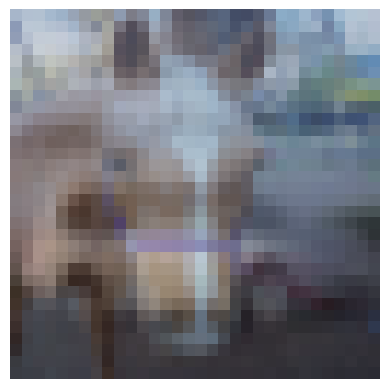
\includegraphics[width=\linewidth]{assets/chapter_4/cifar_rec_lin_comb.png}
    \end{minipage}
    \hfill
    \begin{minipage}{0.31\linewidth}
        \centering
        {Original}
        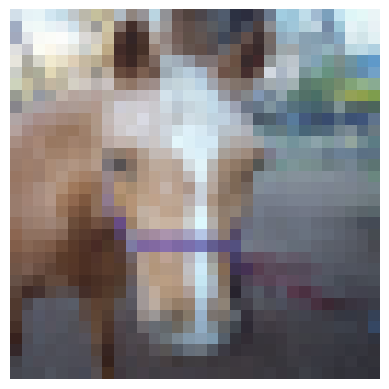
\includegraphics[width=\linewidth]{assets/chapter_4/cifar_rec_2.png}
    \end{minipage}
    \hfill
    \begin{minipage}{0.31\linewidth}
        \centering
        {Original}
        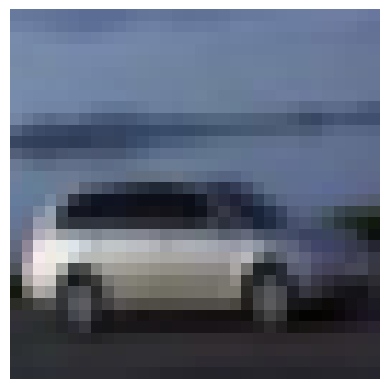
\includegraphics[width=\linewidth]{assets/chapter_4/cifar_rec_1.png}
    \end{minipage}

    \vspace{0.4em}

    \resizebox{\linewidth}{!}{%
        \begin{tabular}{@{}lrrrrr@{}}
            \toprule
            Sample & Bedrooms & Sqft living & Sqft above & Sqft basement & Year built \\
            \midrule
            Reconstruction & 4 & 3215.00 & 2102.00 & 1113.00 & 1998 \\
            Original       & 4 & 2900.00 & 2900.00 & 0.00    & 2005 \\
            Original       & 4 & 3350.00 & 1760.00 & 1590.00 & 1995 \\
            \bottomrule
        \end{tabular}%
    }
    \caption[Original samples and erroneous CTP reconstructions]{Original samples and their erroneous reconstruction by CTP~\cite{ctp_paper}. Top: images from CIFAR-10~\cite{cifar10}. Bottom: tabular records from King County Housing.}
    \label{fig:verification}
\end{figure}

Most existing works evaluate reconstruction performance using reference-based metrics, such as PSNR or SSIM. However, such measures do not provide the attacker with an intrinsic guarantee that a recovered sample corresponds to an original training record in a realistic blind scenario. In vision and language domains, this issue is partially mitigated through human inspection. For example,~\cite{aia_fredrikson} rely on Amazon Mechanical Turk to outsource the image recognition task to human evaluators. Nevertheless, in malicious-server attacks, where the adversary must make decisions during the training phase~\cite{wenFishingUserData2022a,ctp_paper} and may have only limited time between communication rounds to decide which reconstructions to trust and how to adapt subsequent queries, human inspection becomes a costly bottleneck and limits the scalability of the attack. While human assessment may still represent a slow and costly possibility for images, the problem is exacerbated for tabular data, which are central to many federated learning tasks~\cite{ProjectAIKYA, OgierduTerrail2025FedECA}, as numerical values do not offer comparable semantic validation methods~\cite[Figure~1]{veroTabLeakTabularData2023}. As noted by~\citeA[Section~3]{veroTabLeakTabularData2023}, an uninformed adversary may find it nearly impossible to assess reconstruction quality in tabular settings, substantially complicating reliable privacy risk estimation. Figure~\ref{fig:verification} illustrates the difficulty of distinguishing genuine records from erroneous reconstructions, such as combinations of multiple samples, without access to the original data.


To rigorously audit privacy risks in FL, we present in this Chapter a novel reconstruction attack under the malicious-server threat model. By crafting specific model parameters, the server isolates individual samples within an aggregated batch, while our subspace verification test certifies when this isolation has succeeded. This shows that gradient inversion attacks can be more practically dangerous than previously suggested: the attacker can identify correct reconstructions automatically, without human inspection.

Once a sample is certified, our framework analytically recovers its input features and reconstructs the corresponding target value, resulting in a complete breach of the record.

\begin{itemize}
    
    \item We introduce VGIA, the first verifiable gradient inversion attack (VGIA) under a malicious server in FL. VGIA is an analytical  attack that  certifies whether a reconstruction is correct, establishing a more rigorous baseline for privacy auditing than heuristic validation methods.

    \item We empirically validate VGIA on  tabular and image datasets, covering both regression and classification tasks. Our results demonstrate exact record recovery under large-batch aggregation across different data modalities. They also show that VGIA requires fewer attack rounds than previous geometric attacks.
\end{itemize}

\section{Problem Description and Background}\label{sec:vgia_background}

We consider the same federated learning setting described in Section~\ref{sec:fed_learning}. Here, as discussed in Section~\ref{sec:dra}, data reconstruction attacks aim to recover client's private training data. Several appraoch exist, categorized in three main family: optimization-based, generative-based, and analytical-based. 


Across these families, existing attacks still face an important limitation: the attacker may be unable to determine whether a reconstruction corresponds to a single original training record. The reasons for this uncertainty differ across attack families. Analytical attacks may fail to isolate an individual input, producing spurious reconstructions that correspond to linear combinations of multiple samples, according to Equation~\ref{eq:obs_derivation}. Optimization-based attacks, on the other hand, solve a non-convex reconstruction problem, whose optimization may converge to a suboptimal solution that does not faithfully recover the original input, making it difficult to distinguish genuine recoveries from spurious reconstructions. Similarly, generative-model-based attacks may produce inaccurate reconstructions, making it difficult to determine whether the recovered information originates from a single record or combines contributions from multiple samples. Consequently, the attacker may obtain reconstructions that contain information from several training records without being able to identify which candidates correspond to true inputs. The problem can be significant in practice. For example, \citeA[Figure~6]{shan2025geminio} report that more than 35\% of reconstructed samples are spurious for a CIFAR batch of size 256, while \citeA[Table~5]{boenischWhenCuriousAbandon2023} report more than 48\% for an ImageNet batch of size 100.


This raises a fundamental limitation of how GIAs are typically evaluated. Prior work often reports reconstruction quality using reference-based metrics such as SSIM, PSNR, and LPIPS for image data, or BLEU and ROUGE for text data. These metrics require access to the corresponding ground-truth samples and, as noted by~\citeA{veroTabLeakTabularData2023}, do not reflect the attacker's perspective, since the adversary does not have access to the original batch and therefore cannot use them to verify the correctness of individual reconstructions. Moreover, such metrics may not always reflect the actual quality of the recovered information. A reconstruction can obtain a relatively high score while failing to faithfully represent the original input, potentially leading to an inaccurate assessment of the privacy risk posed by the attack. Figure~\ref{fig:scale_mia_rec} illustrates this limitation through reconstructions obtained through the attack proposed by~\cite{shiScaleMIAScalableModel2025} on CIFAR10 data. In the examples shown, representations containing information from multiple samples can achieve relatively high PSNR values, which, according to the reconstruction success criterion adopted in their work, would be classified as correctly recovered samples, despite failing to recover any recognizable input. Consequently, reference-based metrics alone may provide an incomplete assessment of reconstruction success and of the information actually recovered by the attacker.

\begin{figure*}
    \centering 
    % First row
    \subfloat[ResNet\label{fig:non_iso_resnet}]{%
        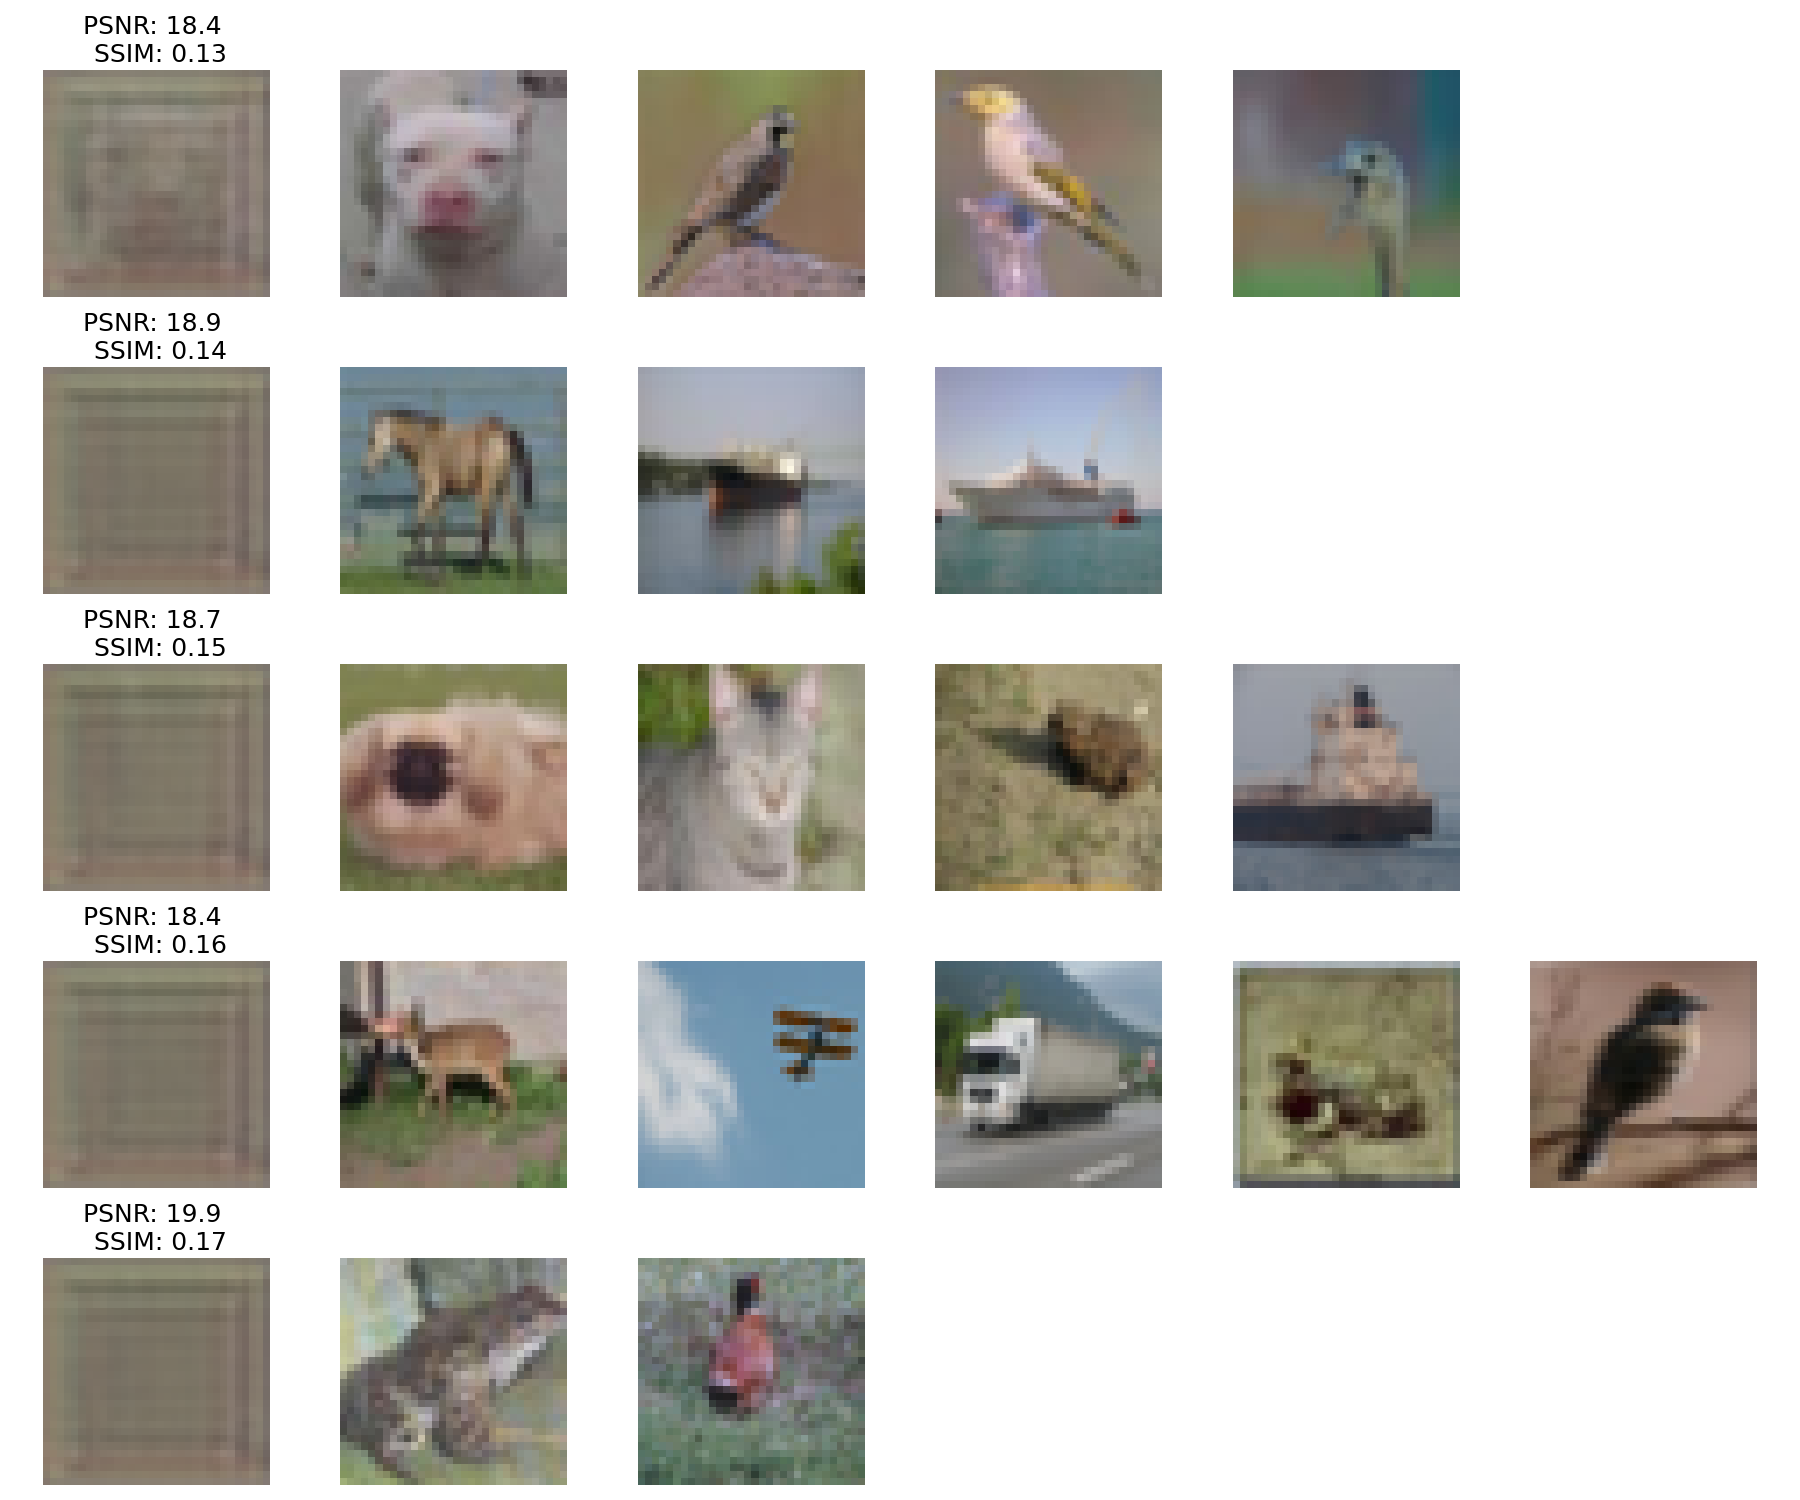
\includegraphics[width=0.47\linewidth]{assets/chapter_4/cifar/non_isolated_psnr_gt_18_Resnet.png}
    }\hspace{0.025\linewidth}
    \subfloat[ViT \label{figures/cifar/non_iso_vit}]{%
        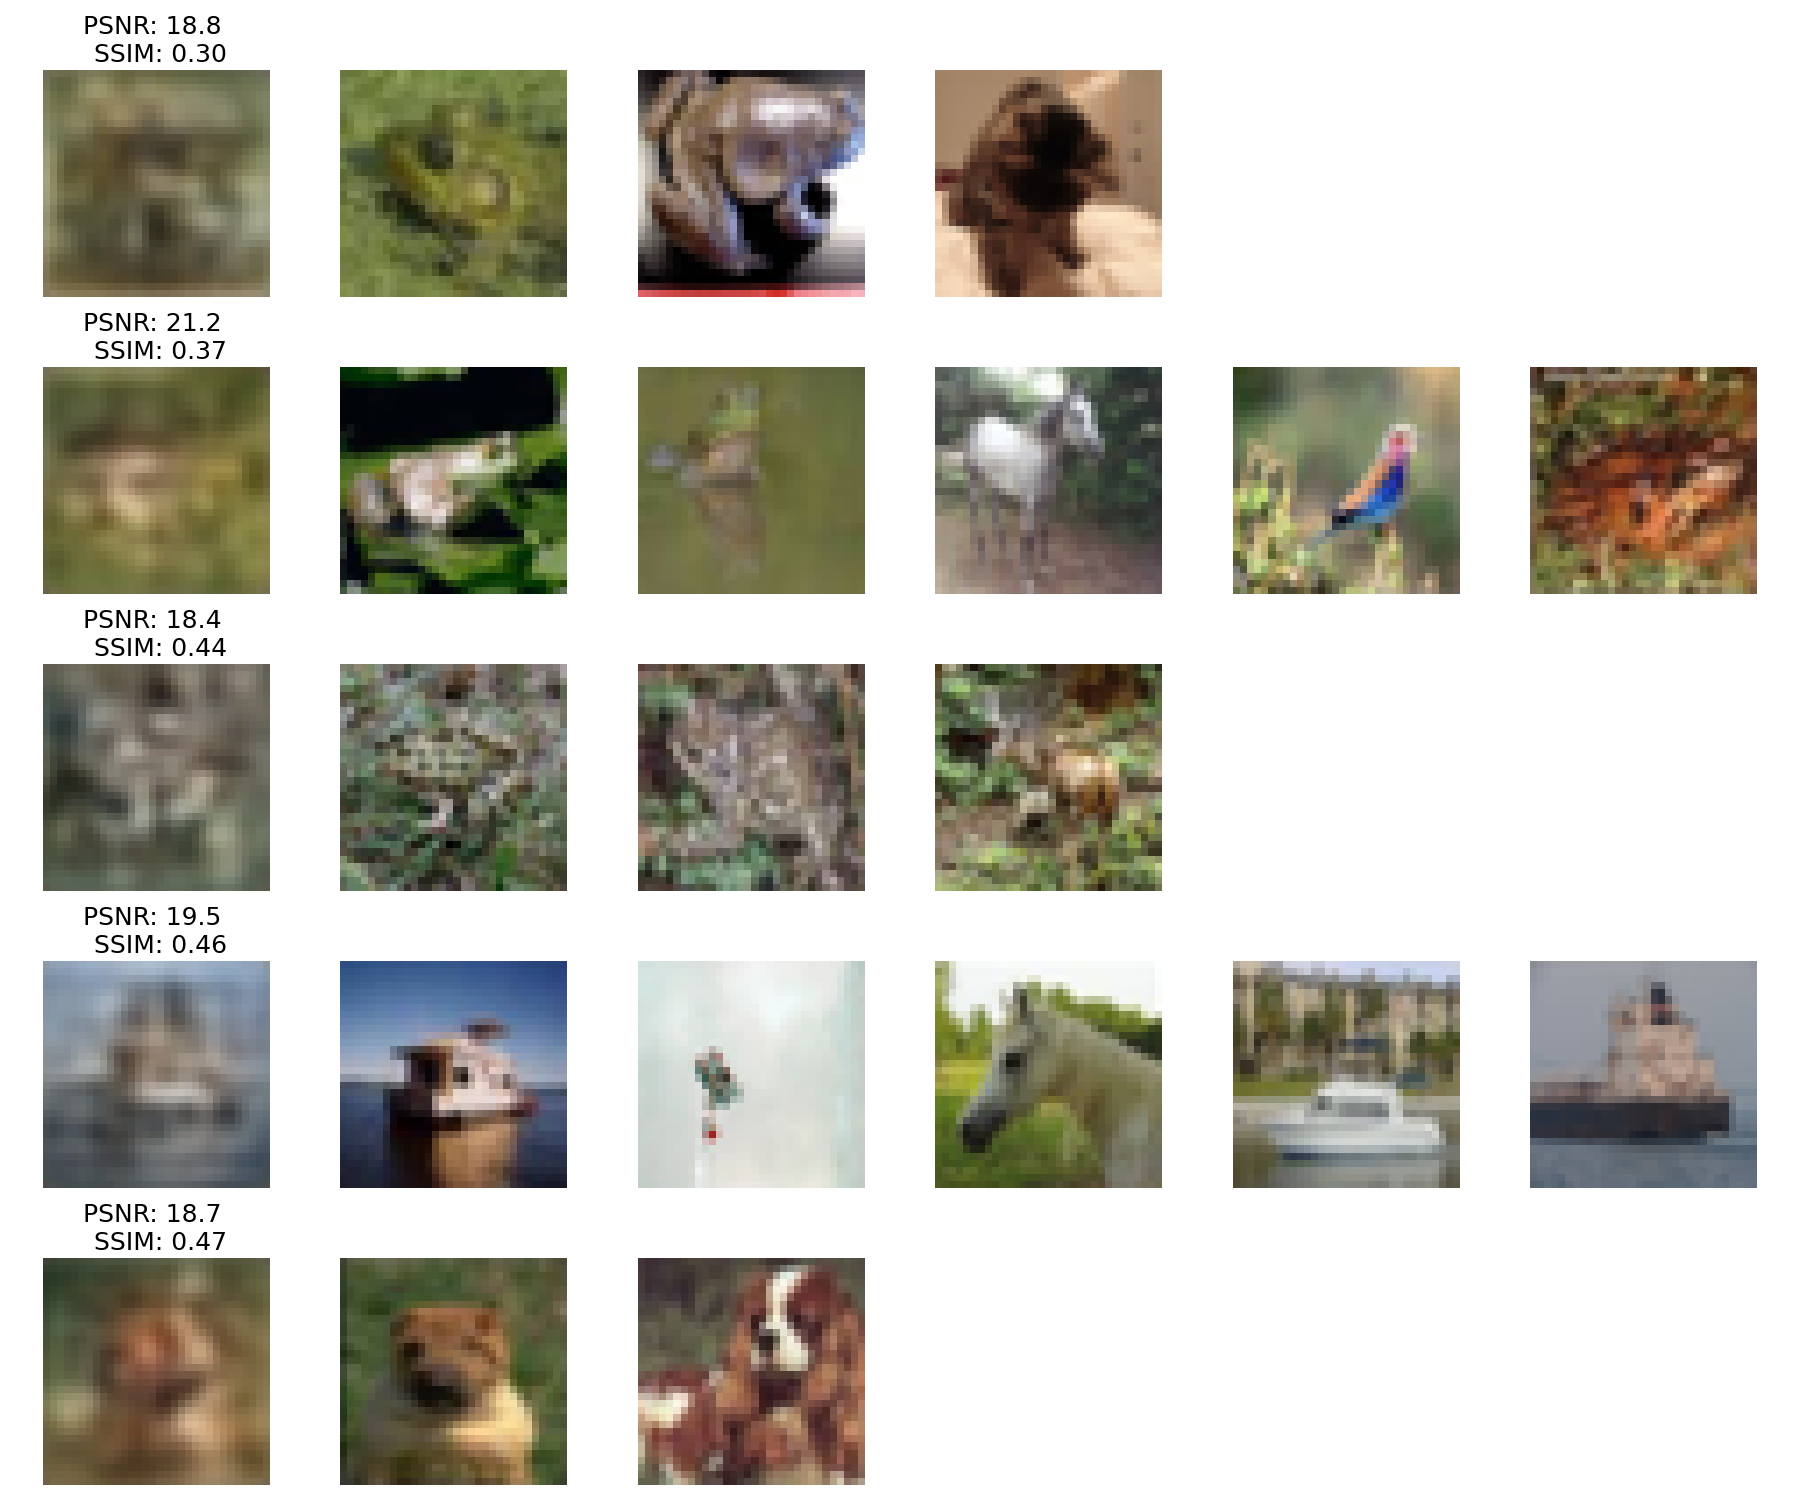
\includegraphics[width=0.47\linewidth]{assets/chapter_4/cifar/non_isolated_psnr_gt_18_Vit.png}
    }\hspace{0.025\linewidth}
    \caption[Scale-MIA reconstruction examples on CIFAR-10]{
    Reconstruction examples from the Scale-MIA attack~\protect\cite{shiScaleMIAScalableModel2025} on a batch of $B=1024$ images from CIFAR-10. The left column shows the decoded image with the corresponding PSNR and SSIM values. The other columns show the corresponding true images isolated in the correspondent bins. In both figures, according to the proposed evaluation metric, the attack is claimed to be successful ($\mathrm{PSNR}>18$). (a) Examples of incorrect isolations from a ResNet model. (b) Examples of incorrect isolations from a ViT model.}
 \label{fig:scale_mia_rec}
    \end{figure*}



Human inspection can sometimes help identify correct reconstructions in image or text data, but it must be performed candidate by candidate and within the limited time window of the attack, making it a costly bottleneck for large batches. For tabular records, manual validation is even more difficult, since numerical values do not provide comparable semantic cues. In particular, a convex combination of continuous features may appear indistinguishable from an actual training sample without access to the original data (Figure~\ref{fig:verification}). The inability to identify genuine recoveries therefore has important implications for the practical privacy risk posed by reconstruction attacks. Even an attack that consistently recovers a small fraction of samples, e.g., $10\%$, can represent a serious privacy threat. However, if the attacker cannot distinguish correctly recovered records from spurious candidates, the reported reconstruction rate may overestimate the amount of private information that the adversary can reliably identify and exploit.


Ideally, GIAs should therefore provide an intrinsic verification mechanism. Despite its practical importance, verifiability has been largely overlooked in the GIA literature; only a few works, mostly in the honest-but-curious setting, offer any form of verification, typically under restrictive conditions.

% \citeA{veroTabLeakTabularData2023} estimate feature-wise reconstruction uncertainty using entropy across reconstructions obtained from repeated, potentially expensive optimization runs. Their assessment is empirically validated, but does not provide formal certificates of reconstruction correctness.
% Analytical attacks from~\cite{dimitrovSPEARExactGradient2024} and \cite{bakarsky2025spearscalinggradientinversion}
% incorporate internal
% reconstruction-validation mechanisms, but require the batch size to be smaller than the input dimension—a restrictive condition for tabular data. 
% Moreover, even in high-dimensional settings that permit large batches, these honest-but-curious methods remain limited in their ability to disentangle increasingly large batches from aggregated gradients.
% %Moreover, these verification mechanisms are tied to honest-but-curious attacks, whose reconstruction performance heavily degrades in large-batch regimes. 
% Finally, in a malicious setting, CTP~\cite{ctp_paper} relies on a stopping
% threshold on the minimum projected
% separation between inputs (see Sec.~\ref{subsec:preliminaries}).



\citeA{veroTabLeakTabularData2023} estimate feature-wise reconstruction uncertainty using entropy across reconstructions obtained from repeated, potentially expensive optimization runs. Thier assessment is empirically validated but does not provide formal certificates of reconstruction correctness, resulting in a costly heuristic rather than a formal guarantee. Analytical attacks from ~\citeA{dimitrovSPEARExactGradient2024} and \citeA{bakarsky2025spearscalinggradientinversion} incorporate internal reconstruction-validation mechanisms, but require the batch size to be smaller than the input dimension—a restrictive condition for tabular data. Moreover, even in high-dimensional settings that permit large batches, these honest-but-curious methods remain limited in their ability to disentangle increasingly large batches from aggregated gradients. In the malicious setting, the Cutting Through Privacy attack developed in Chapter~\ref{chap:ctp} relies on an attacker-detemined tolerance and cannot intrinsically determine whether a sufficiently narrow non-empty region contains one record or several nearby records. Its success criterion therefore depends on an unknown separation between client samples and does not provide a per-reconstruction certificate. (see Section~\ref{subsec:preliminaries}).

\section{A Verifiable Gradient Inversion Attack}
\subsection{Threat Model}\label{sec:vgia_threat_model}
VGIA follows the same malicious server setting described in Section~\ref{sec:threat}, consistent with the CTP attack setting.

The server is not allowed to modify the model architecture, for example by adding layers or modules~\cite{fowlRobbingFedDirectly2021,fowlDecepticonsCorruptedTransformers2022,zhaoLOKILargescaleData2023a,shiScaleMIAScalableModel2025}, changing internal connections or routing mechanisms~\cite{fowlDecepticonsCorruptedTransformers2022,chu2023panning}, or altering activation functions~\cite{fowlRobbingFedDirectly2021}. Second, we do not assume access to auxiliary or public datasets, unlike~\cite{boenischWhenCuriousAbandon2023,ZHANG2023119421,garovHidingPlainSight2024,shiScaleMIAScalableModel2025}, nor auxiliary knowledge of the data distribution unlike~\cite{fowlRobbingFedDirectly2021,fowlDecepticonsCorruptedTransformers2022,shiScaleMIAScalableModel2025}.
As in CTP, we assume that the inputs lie in a bounded domain and that the attacker knows only lower and upper bounds on each input feature after preprocessing.

In the following, we focus on clients updating the global model with full-batch FedSGD. We also extend the attack to FedAvg in Section~\ref{sec:fedavg_vgia} and empirically evaluate it in Section~\ref{sec:fedavg_vgia_exp}.

\subsection{Preliminaries}\label{subsec:preliminaries}
Our work builds upon the fundamental observation that the gradients of a fully connected (FC) layer followed by a ReLU activation can encode sufficient information to analytically reconstruct the layer inputs, as described in Section~\ref{sec:ctp_background}. 
To recall the undeline machanism, consider a model whose first (attacked) layer is a linear layer with $N$ neurons, parameterized by weights $\W^a \in \mathbb{R}^{N \times d}$ and biases $\b^a \in \mathbb{R}^N$. For neuron $i$, the post-activation output is
\[
z_i^a = \mathrm{ReLU}\!\left(\W_i^a \x + b_i^a\right),
\]
where $\x \in \mathbb{R}^d$ denotes the input to the attacked layer. As shown in Equation~\ref{eq:aggr_obs}, the attacker can retrieve a linear combination of the batch inputs, where only samples that activate neuron $i$ have a nonzero coefficient $\alpha_j$, and therefore contribute to $\o_i$. Disentangling individual samples from the aggregate $\o_i$ is the central challenge in analytic gradient inversion.

To address the limitations of existing reconstruction attacks, the previous chapter introduced a geometric interpretation of ReLU-based leakage, detailed in Section~\ref{sec:limit}, which motivated the CTP attack presented in Section~\ref{sec:our_attack}. By interpreting ReLU activation boundaries as hyperplanes, CTP progressively partitions the input space into slices, identifies regions containing client inputs, and reconstructs individual samples from their gradient contributions.

CTP can identify empty slices and discard them from subsequent queries, but it cannot determine whether a non-empty slice contains a single sample or multiple samples. As a result, every non-empty slice is recursively bisected until its width falls below a user-defined threshold \(\varepsilon\). This stopping criterion introduces two limitations. First, if two inputs have projections along the normal direction of \(\W_i^a\) that differ by less than \(\varepsilon\), CTP may terminate before separating them, leading to an incorrect reconstruction. Second, setting \(\varepsilon\) unnecessarily small increases the number of communication rounds, since the attack continues refining slices that may already contain a single sample. Figure~\ref{fig:ctp_ok} illustrates a successful case in which CTP recovers three inputs after 6 rounds, using 3 hyperplanes per round and 18 hyperplanes in total. Figure~\ref{fig:ctp_miss}, instead, illustrates a failure case in which two inputs remain within the same \(\varepsilon\)-wide slice and cannot be separated. Under a realistic blind threat model, the adversary does not know the distances between sample projections in advance and therefore cannot select \(\varepsilon\) reliably.


\begin{figure}[tb]
    \centering
    % All four subfloats on the same line
    \subfloat[\label{fig:ctp_ok}]{%
        \includegraphics[width=0.23\linewidth]{assets/chapter_4/search_example/ctp_example.pdf}
    }\hfill 
    \subfloat[\label{fig:new_ok}]{%
        \includegraphics[width=0.23\linewidth]{assets/chapter_4/search_example/new_example.pdf}
    }\hfill
    \subfloat[\label{fig:ctp_miss}]{%
        \includegraphics[width=0.23\linewidth]{assets/chapter_4/search_example/ctp_example_miss.pdf}
    }\hfill
    \subfloat[\label{fig:new_adv}]{%
        \includegraphics[width=0.23\linewidth]{assets/chapter_4/search_example/new_example_miss.pdf}
    }

    \caption{A two-dimensional example of the search process. Figure~\ref{fig:ctp_ok} illustrates the CTP process, while Figure~\ref{fig:new_ok} depicts VGIA method. In this instance, VGIA requires fewer rounds than their approach, as we avoid searching up to $\varepsilon$ distance across the entire space. Conversely, when $\varepsilon$ is not well-tuned, Figure~\ref{fig:ctp_miss} shows that the CTP attack fails, whereas VGIA (Figure~\ref{fig:new_adv}) continues searching until all data points are exactly separated.}
    \label{fig:main_fig}
\end{figure}

\subsection{Verifiable Isolation and Reconstruction}\label{sec:attack_method}

VGIA addresses the two main limitations of CTP. First, it introduces an algebraic verification step that allows the attacker to certify when a slice contains a single input. Second, once a slice has been certified, VGIA removes it from further refinement and reallocates future hyperplane queries to unresolved regions. This avoids unnecessary dissections of already isolated samples and reduces the number of communication rounds required for full-batch reconstruction. 

Figure~\ref{fig:new_ok} illustrates that, by correctly identifying slices that contain a single input, VGIA reconstructs all samples in only $4$ rounds ($12$ hyperplanes), compared to $6$ rounds ($18$ hyperplanes) for CTP (Figure~\ref{fig:ctp_ok}). Moreover, Figure~\ref{fig:new_adv} shows that VGIA's protocol adapts the number of rounds and hyperplanes to the specific batch: in this example it continues for $8$ rounds to isolate all inputs, whereas CTP (Fig.~\ref{fig:ctp_miss}) stops too early and produces an incorrect reconstruction.

We first present VGIA for an $L$-layer fully connected neural network with a single scalar output and ReLU activations. In this setting, the attacked first layer is parameterized by weights $\W^a \in \real^{N\times d}$ and biases $\b^a \in \real^N$, and is followed by a ReLU activation. The last layer is parameterized by weights $\W^L \in \real^{1 \times M}$ and bias $b^{L} \in \real$, where $M$ denotes the number of neurons in layer $L-1$.

Extensions to multi-dimensional output, to FedAvg, to different activation functions such as SiLU and GELU, and to other architectures including convolutional neural networks and transformers are provided in Sections~\ref{sec:multiclass_vgia},~\ref{sec:fedavg_vgia},~\ref{sec:silu_gelu}, and \ref{sec:scalemia_comparison}, respectively. For FedAvg and smooth activations such as SiLU and GELU, our verification is approximate. For CNNs and Transformers, the guarantees apply to suitable intermediate embeddings, while reconstructing the original inputs requires a decoder, as in~\citeA{shiScaleMIAScalableModel2025}.



\subsubsection{Verifiable Isolation}
The first step of our attack is to extract the contribution of the inputs lying between two consecutive hyperplanes.

Within a single round, the attacker can test multiple parallel hyperplanes with normal vector $\mathbf w$ by targeting different neurons and setting their weight vectors to $\mathbf w$ (e.g., $\W_i^a=\W_{i'}^a=\mathbf w$ for two targeted neurons $i$ and $i'$), while assigning the corresponding neurons different biases (so $b_i^a \neq b_{i'}^a$). For simplicity, we assume that all neurons in the layer are targeted.


We first analyze the gradient of the loss with respect to neuron $i$'s weights  $\gradlosswiatt$.
\begin{align}
    \gradlosswiatt &= \frac{1}{B} \sum_{j=1}^B \frac{\partial \loss_j}{\partial z_{i}^a}\, \x_j\, \indicator_{z_{i,j}^a>0} = \frac{1}{B} \sum_{j \in \activeset_i} \frac{\partial \loss_j}{\partial z_{i}^a}\, \x_j
    =\frac{1}{B} \sum_{j \in \activeset_i}
    \frac{\partial \loss_j}{\partial z^L}\frac{\partial z^L}{\partial z_i^a}\x_j, \label{eq:weight_gradient}
\end{align}

where the indicator function $ \indicator_{z_{i,j}>0}$ specifies whether neuron $i$ is activated by sample $\x_j$, B is the batch size, and $\activeset_i = \{j \in [B] \mid \W_i^a \x_j + b_i^a > 0\}$ denotes the set of indices that activate neuron $i$. 

In general, the  partial derivative $\frac{\partial z^L}{\partial z_i^a}$  
%from the network output to neuron $i$ in layer $a$ 
depends on the input $\x$, because downstream ReLU gates may switch on/off as $\x$ changes. 
%Concretely, $\frac{\partial z^L}{\partial z_i^a}(\x)$ is typically $\x$-dependent. 
However, the malicious server can choose the parameters of the subsequent layers $(\W^{a+1:L}, \b^{a+1:L})$, so
that the activation pattern of all ReLUs after layer $a$ is fixed for all inputs of interest.
Once this is achieved, $z^L$ becomes an affine function of $z^a$, and the server can ensure that the Jacobian entry $\frac{\partial z^L}{\partial z_i^a}$ is a nonzero constant, denoted by $g_i$.

A simple way to enforce input-independent downstream gating, when the layer inputs are non-negative, is to use positive weights and biases in the subsequent layers, so that all downstream pre-activations remain positive and all ReLUs are always active. This construction provides a convenient sufficient condition for the attack, but such a strict configuration is not necessary. More generally, a malicious server can design the parameter modifications so that the gradient contributions preserve the algebraic structure required for reconstruction, while using parameter configurations that are less distinguishable from benign training. 

For example, the attacker can sample weights and biases from realistic-looking distributions while enforcing a prescribed activation pattern, or manipulate only a subset of neurons and constrain their outgoing connections so that neuron-dependent factors can be normalized out. A more detailed discussion of these constructions and their impact on attack detectability is provided in Section~\ref{sec:detectability}.

Consider two consecutive bias values $\hat b_k < \hat b_{k+1}$ tested at two attacked neurons in the same round. Without loss of generality, assume these neurons are $i$ and $i+1$. We call the region delimited by the two hyperplanes $(\mathbf w,\hat b_k)$ and $(\mathbf w,\hat b_{k+1})$ the \emph{$k$-th slice}.

Dividing~\eqref{eq:weight_gradient} by the constant $g_i$ and subtracting it from the corresponding expression for neuron $i+1$, the server obtains the \emph{slice vector} $\slice_k$, a linear combination of the inputs lying in the slice between the two corresponding hyperplanes:
\begin{align}
   \slice_k &=  \frac{\frac{\partial \loss}{\partial \W_{i+1}^a}}{g_{i+1}} - \frac{\frac{\partial \loss}{\partial \W_{i}^a}}{g_i} = \frac{1}{B} \sum_{\x_j \in \activeset_{i+1}} \frac{\partial \loss_j}{\partial z^{L}} \x_j - \frac{1}{B} \sum_{\x_j \in \activeset_{i}} \frac{\partial \loss_j}{\partial z^{L}} \x_j  = \frac{1}{B} \sum_{j \in \activeset_{i+1} \setminus \activeset_{i} 
    } \frac{\partial \loss_j}{\partial z^{L}} \x_j \label{eq:hp_diff}.
\end{align}

This quantity is computable by the server, which observes the client gradient and knows the constants $g_i$ and $g_{i+1}$. The rescaling is essential to the construction because it removes the architecture-dependent factors from the gradient observations. Consequently, when the rescaled gradients of two consecutive neurons are subtracted, the contributions of samples activating both neurons cancel exactly in~\eqref{eq:hp_diff}, leaving only the contribution of samples located between the corresponding hyperplanes. Without rescaling, the factors $g_i$ and $g_{i+1}$ would generally differ, preventing this cancellation and leaving residual contributions from samples in $\activeset_i$.

The resulting slice vector therefore directly indicates whether the interval between the two hyperplanes contains any data. If $\activeset_i$ coincides with $\activeset_{i+1}$, no sample lies in the interval and the corresponding slice vector is zero. The server can discard such empty slices and, in subsequent rounds, place new hyperplanes only within intervals associated with nonempty slice vectors. In this way, the attack progressively prunes empty regions of the search space and concentrates its queries on intervals that contain client samples.

The key remaining question is whether a nonzero slice vector corresponds to a single input or to a combination of several inputs. To answer this question, the attacker refines a non-empty slice by placing $q\ge 3$ hyperplanes across it. The resulting $q-1$ sub-slice vectors allow the attacker to certify whether all samples in the parent slice have been isolated. Formally, consider a non-empty slice at round $t$, delimited by the bias values $\hat b_k^{t}$ and $\hat b_{k+1}^{t}$, with slice vector $\slice_k^t$. At round $t+1$, the attacker places $q$ bias values in $[\hat b_k^{t}, \hat b_{k+1}^t]$, that is
$
\hat b_{k}^{t+1} = \hat b_{k}^{t}
< \hat b_{k+1}^{t+1}
< \cdots
< \hat b_{k+q-1}^{t+1}
= \hat b_{k+1}^{t},
$
and computes the induced sub-slice vectors $\slice_k^{t+1}, \slice_{k+1}^{t+1}, \dots, \slice_{k+q-2}^{t+1}$. If $\slice_k^t$ is contained in the span of these $q-1$ sub-slice vectors, then each non-empty sub-slice contains exactly one sample, as stated in the following proposition.

\begin{proposition}[Verifiable isolation]
\label{prop:sample_isolation}
Consider the non-empty slice delimited at round $t$ by the hyperplanes
$\mathbf w^\top \x+\hat b_k^t=0$ and $\mathbf w^\top \x+\hat b_{k+1}^t=0$,
and suppose that it contains $m\le d$ linearly independent inputs. Assume that
the common first-layer direction $\mathbf w$ is drawn once from a distribution
absolutely continuous with respect to the Lebesgue measure. At each attack round,
assume that the vectorized weights and biases of the layers following the
attacked layer are redrawn independently of the past from absolutely continuous
distributions, supported on parameters for which each downstream hidden layer
has at least two fixed ReLU gates active on all inputs in the slice. Finally,
assume that, for every sample $j$, all level sets of
$\partial \loss_j/\partial z^L$ are Lebesgue-null.

Then, almost surely, the span condition
\[
\slice_k^t
\in
\operatorname{span}\left(
\slice_k^{t+1},\ldots,\slice_{k+q-2}^{t+1}
\right)
\]
implies that every non-empty sub-slice induced at round $t+1$ contains exactly
one input. Hence, when the span condition holds, the original slice contains
as many inputs as there are non-null induced slice vectors, and therefore at
most $q-1$ inputs.
\end{proposition}

Proposition~\ref{prop:sample_isolation} provides the criterion used by VGIA to decide whether a slice has been fully resolved. If the span condition holds, each non-empty induced sub-slice contains a single input and can be reconstructed as described below. If the condition does not hold, the slice remains unresolved and is further refined in subsequent rounds.

Note that the assumptions underlying Proposition~\ref{prop:sample_isolation} concern only the slice being verified. In particular, linear independence is required among the inputs contained in that slice, not across the entire batch. The condition on $\frac{\partial \loss_j}{\partial z^L}$ is also satisfied by any loss whose derivative varies with the activation value, such as the logistic, exponential, focal, and squared losses. Since VGIA progressively partitions the batch into increasingly small subsets, the linear-independence condition can remain applicable even when the batch size greatly exceeds the input dimension.

For example, in the experiments of Section~\ref{sec:exp_results}, VGIA successfully attacks batches of $B=2048$ samples with $N=1000$ neurons on low-dimensional datasets such as King County Housing~\cite{kingcountyhousing}, which has only $d=18$ input features. After the initial partition, each slice contains approximately two samples on average. The linear-independence condition therefore needs to hold only within these small local subsets, even though the full batch contains far more than $d$ samples.

Even when linear independence is violated within a slice, an incorrect certification does not necessarily follow. If the span condition fails, VGIA continues refining the slice, and the smaller subsets produced in subsequent rounds may satisfy the assumption. A failure can occur only if the span condition is satisfied while one of the induced sub-slices still contains multiple samples, in which case the resulting reconstruction may be a linear combination of those inputs. Such a failure remains local to the affected slice and does not compromise the verification of other regions of the search space.
 

Figure~\ref{fig:vgia_isolation_sequence} illustrates the search process over three
consecutive rounds, separating the geometry of the queried slices from the
subspace test performed on the observed gradients.
\francesco{adjust the figure down right }
\begin{figure}[!htbp]
    \centering
    \resizebox{\linewidth}{!}{% A static animation: read columns left to right, with the same two inputs
% and the same input-space coordinates in every frame. The vector-space
% sketches below are schematic; coefficients may change between rounds.
\begingroup
\definecolor{vgiablue}{HTML}{276B91}
\definecolor{vgiaamber}{HTML}{B96720}
\definecolor{vgiagreen}{HTML}{247C68}
\definecolor{vgiaviolet}{HTML}{79519A}
\definecolor{vgiagray}{HTML}{75818B}
\begin{tikzpicture}[x=1cm,y=1cm,>=stealth,
  every node/.style={font=\small},
  boundary/.style={draw=vgiablue,line width=1pt},
  newcut/.style={draw=vgiablue,dashed,line width=1.1pt},
  sample/.style={circle,fill=black!75,inner sep=2pt},
  recovered/.style={circle,draw=vgiagreen,fill=vgiagreen!15,line width=1pt,inner sep=2.5pt},
  note/.style={align=center,text width=4.1cm,font=\footnotesize},
  % Match each lower plotting area to the upper panels: 4.2 by 2.7 cm.
  verification panel/.style={xscale=1.2727272727,yscale=1.2},
  vec/.style={->,line width=1.2pt}]
  \foreach \offset/\heading in {0/{(a) Round $t$},4.65/{(b) Round $t+1$},9.3/{(c) Round $t+2$}} {
    \node[font=\small\bfseries] at (\offset+2.1,7.4) {\heading};
  }
  % \node at (2.1,6.95) {Observe a non-empty slice};
  % \node at (6.75,6.95) {Refine, then test};
  % \node at (11.4,6.95) {Split again, then certify};
  \draw[->,thick,black!40] (4.02,7.4)--(4.62,7.4);
  \draw[->,thick,black!40] (8.67,7.4)--(9.27,7.4);

  % INPUT SPACE. All boundaries satisfy x + .18 y = constant;
  % hence w = (1,.18) is normal to every tilted hyperplane.
  % Successive midpoint cuts: .543 and 4.143 -> 2.343;
  % then 2.343 and 4.143 -> 3.243 (bottom-edge coordinates).
  \begin{scope}[yshift=3.8cm]
    \fill[vgiaamber!13] (.543,0)--(4.143,0)--(3.657,2.7)--(.057,2.7)--cycle;
    \draw[boundary] (.543,0)--(.057,2.7);
    \draw[boundary] (4.143,0)--(3.657,2.7);
    \node[text=vgiaamber] at (2.1,1.45) {$\slice_k^t$};
  \end{scope}
  \begin{scope}[xshift=4.65cm,yshift=3.8cm]
    \fill[black!4] (.543,0)--(2.343,0)--(1.857,2.7)--(.057,2.7)--cycle;
    \fill[vgiaamber!13] (2.343,0)--(4.143,0)--(3.657,2.7)--(1.857,2.7)--cycle;
    \draw[boundary] (.543,0)--(.057,2.7);
    \draw[boundary] (4.143,0)--(3.657,2.7);
    \draw[newcut] (2.343,0)--(1.857,2.7);
    \node[text=vgiagray] at (1.05,1.4) {$\slice_{k+1}^{t+1}$};
    \node[text=vgiaamber] at (3.05,1.45) {$\slice_k^{t+1}$};
  \end{scope}
  \begin{scope}[xshift=9.3cm,yshift=3.8cm]
    \fill[black!4] (.543,0)--(2.343,0)--(1.857,2.7)--(.057,2.7)--cycle;
    \fill[vgiagreen!10] (2.343,0)--(3.243,0)--(2.757,2.7)--(1.857,2.7)--cycle;
    \fill[vgiagreen!20] (3.243,0)--(4.143,0)--(3.657,2.7)--(2.757,2.7)--cycle;
    \draw[vgiagray,dotted] (.543,0)--(.057,2.7);
    \draw[boundary] (2.343,0)--(1.857,2.7);
    \draw[boundary] (4.143,0)--(3.657,2.7);
    \draw[newcut] (3.243,0)--(2.757,2.7);
    \node[text=vgiagray] at (1.05,1.4) {$\slice_{k+1}^{t+1}$};
    \node[text=vgiagreen,font=\footnotesize] at (2.54,1.4) {$\slice_{k+1}^{t+2}$};
    \node[text=vgiagreen,font=\footnotesize] at (3.44,1.4) {$\slice_k^{t+2}$};
  \end{scope}
  \foreach \offset in {0,4.65,9.3} {
    \begin{scope}[xshift=\offset cm,yshift=3.8cm]
      \draw[black!20] (0,0) rectangle (4.2,2.7);
      % \draw[vec,vgiablue] (.55,2.05)--(1.3,2.185)
      %   node[above,font=\footnotesize] {$\mathbf w$};
      \node[sample] at (2.6,.6) {};
      \node[sample] at (3.4,2.3) {};
      \node[anchor=north,font=\footnotesize] at (2.6,.48) {$\x_1$};
      \node[anchor=north,font=\footnotesize] at (3.4,2.18) {$\x_2$};
    \end{scope}
  }

  \begin{scope}[verification panel]
    \draw[->,black!25] (0,0)--(3.3,0);
    \draw[->,black!25] (0,0)--(0,2.25);
    \draw[vec,vgiaamber] (0,0)--(2.6,.85) node[above] {$\slice_k^t$};
    \node[note] at (1.65,-.55)
      {$\slice_k^t=\beta_1^t\x_1+\beta_2^t\x_2$};
    % \node[note,text=vgiaamber] at (1.65,-1.2)
    %   {Not yet certified.};
  \end{scope}
  \begin{scope}[xshift=4.65cm,verification panel]
    \draw[->,black!25] (0,0)--(3.3,0);
    \draw[->,black!25] (0,0)--(0,2.25);
    \draw[vgiablue!45,line width=4pt] (0,0)--(3.25,1.56);
    \draw[vec,vgiablue] (0,0)--(2.5,1.2) node[right] {$\slice_k^{t+1}$};
    \draw[vec,vgiaamber] (0,0)--(2.6,.85) node[right] {$\slice_k^t$};
    \node[note] at (1.65,-.55)
      {$\slice_k^t\notin\operatorname{span}\{\mathbf 0,\slice_k^{t+1}\}$};
    % \node[note,text=vgiaamber] at (1.65,-1.2)
    %   {Fail: refine again.};
  \end{scope}
  \begin{scope}[xshift=9.3cm,verification panel]
    % \fill[vgiagreen!8] (0,0) rectangle (3.3,2.25);
    % R = A + B, with A = a s_{k+1}^{t+2}, B = b s_k^{t+2}.
    % Coefficients for this schematic: a=.6887676692, b=.7556603942.
    \coordinate (sumA) at (1.10202827,.25431369);
    \coordinate (sumB) at (1.39797173,.94568631);
    \coordinate (sumR) at (2.5,1.2);
    % \fill[vgiagreen!17] (0,0)--(sumA)--(sumR)--(sumB)--cycle;
    \draw[->,black!25] (0,0)--(3.3,0);
    \draw[->,black!25] (0,0)--(0,2.25);
    \draw[vec,vgiagreen] (0,0)--(1.6,.36923) node[below] {$\slice_{k+1}^{t+2}$};
    \draw[vec,vgiaviolet] (0,0)--(1.85,1.25147) node[above left] {$\slice_k^{t+2}$};
    \draw[->,dashed,line width=1pt,vgiagreen] (sumB)--(sumR)
      node[midway,above,font=\footnotesize] {$a\slice_{k+1}^{t+2}$};
    \draw[->,dashed,line width=1pt,vgiaviolet] (sumA)--(sumR)
      node[midway,right,font=\footnotesize] {$b\slice_k^{t+2}$};
    \draw[vec,vgiablue] (0,0)--(sumR) node[right] {$\slice_k^{t+1}$};
    \node[note] at (1.65,-.55)
      {$\slice_k^{t+1}=\textcolor{vgiagreen}{a\slice_{k+1}^{t+2}}+\textcolor{vgiaviolet}{b\slice_k^{t+2}}$};
    % \node[note,text=vgiagreen] at (1.65,-1.2)
    %   {Pass: two singletons.};
  \end{scope}
  % True input vectors: one common display scale (.85) in all three panels.
  % In the last frame, shorter green vectors lie on these same two rays.
  \foreach \offset in {0,4.65,9.3} {
    \begin{scope}[xshift=\offset cm,verification panel]
      \draw[->,dashed,black!60,line width=.8pt] (0,0)--(2.21,.51)
        node[below right,font=\footnotesize,text=black!75] {$\x_1$};
      \draw[->,dashed,black!60,line width=.8pt] (0,0)--(2.89,1.955)
        node[above,font=\footnotesize,text=black!75] {$\x_2$};
    \end{scope}
  }
  % \draw[black!15] (0,-1.8)--(13.5,-1.8);
  % \node[align=center,font=\small,text=vgiagreen] at (6.75,-2.25)
  %   {\textbf{Recover and stop refining:}\quad
  %   $\displaystyle \x_1=\frac{\slice_{k+1}^{t+2}}{\beta_1^{t+2}},\qquad
  %   \x_2=\frac{\slice_k^{t+2}}{\beta_2^{t+2}}$};
  % \node[font=\footnotesize,text=vgiagray] at (6.75,-3.2)
  %   {The bias-gradient differences give $\beta_1^{t+2}$ and $\beta_2^{t+2}$ via~\eqref{eq:rec_coeff}.};
\end{tikzpicture}
\endgroup
}
    \caption[Step-by-step isolation and verification in VGIA]{VGIA isolation and verification for two inputs in $\real^2$. The top row shows successive search rounds. The bottom row shows the corresponding slice vectors: verification fails while both inputs share a sub-slice, then succeeds when $\slice_k^{t+1}\in\operatorname{span}\{\slice_{k+1}^{t+2},\slice_k^{t+2}\}$.}
    \label{fig:vgia_isolation_sequence}
\end{figure}

\subsubsection{Reconstruction}
Once an isolated slice has been identified, the attacker can recover the corresponding input directly. Suppose that the slice vector $\slice_k^{t+1}$, obtained from the two hyperplanes tested at neurons $i$ and $i+1$, contains a single input $\x_j$. From~\eqref{eq:hp_diff}, we have
$\slice_k^{t+1} = \beta_j^{t+1}\x_j$, where
$\beta_j^{t+1} \coloneqq \frac{1}{B}\frac{\partial \loss_j}{\partial z^{L}}$.
Recovering $\x_j$ therefore only requires estimating the scalar $\beta_j^{t+1}$.
This coefficient can be obtained from the gradients with respect to the attacked-layer biases. Expanding $\frac{\partial \loss}{\partial b_i^a}$ as in~\eqref{eq:weight_gradient} and applying the same rescaling and subtraction as in~\eqref{eq:hp_diff} gives
\begin{equation}
\frac{\frac{\partial \loss}{\partial b_{i+1}^a}}{g_{i+1}}
-
\frac{\frac{\partial \loss}{\partial b_i^a}}{g_i}  =
\frac{1}{B} \sum_{\ell \in \activeset_{i+1}}
\frac{\partial \loss_\ell}{\partial z^{L}}
-
\frac{1}{B} \sum_{\ell \in \activeset_i}
\frac{\partial \loss_\ell}{\partial z^{L}}  =
\frac{1}{B}
\sum_{\ell \in \activeset_{i+1} \setminus \activeset_i}
\frac{\partial \loss_\ell}{\partial z^{L}} = \frac{1}{B}\frac{\partial \loss_j}{\partial z^{L}} = \beta_j^{t+1}.
\label{eq:rec_coeff}
\end{equation}
Using Equations~\eqref{eq:hp_diff} and~\eqref{eq:rec_coeff}, the attacker therefore recovers the private input exactly as
$\hat{\x}_j=\slice_k^{t+1}/\beta_j^{t+1}=\x_j$. 

Once the input has been reconstructed, the attacker can also recover its corresponding target $y_j$. 
In classification tasks, target inference has been widely studied~\cite{yinSeeGradientsImage2021,zhaoIDLGImprovedDeep2020,kariyappaCocktailPartyAttack2023,liE2EGIEndtoEndGradient2023}, where the finite set of possible labels makes it possible to evaluate a discrete set of candidates.
The problem is different for regression, where the target is continuous and cannot be inferred by testing a finite set of candidate values. In VGIA, Equation~\eqref{eq:rec_coeff} provides the attacker with the derivative associated with the isolated sample,
\[
\frac{\partial \loss_j}{\partial z^L} = B\beta_j^{t+1}.
\]

This derivative is evaluated on the true pair $(\x_j,y_j)$ and therefore contains information about the unknown target $y_j$. Since the input $\x_j$ has already been reconstructed and the model parameters are known by the attacker, the server can then evaluate, for a candidate value $y$, the derivative that would be produced by the pair $(\x_j,y)$. Target reconstruction can therefore be formulated as the following univariate optimization problem:
\begin{equation}
\hat{y}_j \in
\argmin_y
\left(
B\beta_j^{t+1}
-
\frac{\partial \loss}{\partial z^L}(\x_j,y)
\right)^2.
\label{eq:target_rec}
\end{equation}
If the derivative of the loss with respect to the network output is monotone in $y$, as for the squared loss, Problem~\eqref{eq:target_rec} admits a unique solution, allowing the attacker to reconstruct the complete private record $(\x_j,y_j)$. 

\subsection{Final Algorithm}

Algorithm~\ref{algo:vgia_parallelattack} presents the full VGIA procedure. As assumed in Section~\ref{sec:vgia_threat_model}, the attacker knows bounds on the input features. These bounds induce an initial interval $[l,u]$ for the projections $\mathbf w \x$, and therefore for the bias values to be queried.
The procedure \textsc{SetHyperplanes} (Algorithm~\ref{algo:set_hp_biases}) constructs the $N$ hyperplanes queried by the attacker, one per attacked neuron. During the first communication round, the biases associated with each hyperplanes partition the initial search interval $[l,u]$ into $N-1$ slices. From the second round onward, each selected interval is queried with at least three hyperplanes, including its two boundary hyperplanes and at least one new interior hyperplane. The boundary hyperplanes must be queried again at each round to compute the new slice vectors, because, unlike CTP, the parameters $\W^{a+1:L}$ are not required to remain fixed throughout the attack and can be updated between rounds to make the attack less detectable (Section~\ref{sec:detectability}). 

Consequently, the gradients associated with the same neuron in~\eqref{eq:weight_gradient} may vary across rounds.
The procedure \textsc{CheckIsolation} in Algorithm~\ref{algo:check_isolation} uses Proposition~\ref{prop:sample_isolation} to certify when a slice contains exactly one sample. Certified slices are added to $\mathcal R$ and are ready for reconstruction. The same procedure also detects empty slices through a null slice vector, in which case the corresponding interval is discarded.

%Theoretically, 
\subsection{Round Complexity}\label{sec:round_complexity_vgia}
\francesco{Verify and integrate the new proof}
 Under the same assumptions of Proposition~\ref{prop:sample_isolation},
if $N \geq 3B$, our algorithm can verify all inputs in a batch with high probability in at most
$
3 \cdot \left\lceil \log_2 \left(\frac{W}{N \cdot \eps_{\mathbf w}}\right) \right\rceil + 1
$
rounds, where $\eps_{\mathbf w}$ is the minimum distance between two samples after projection onto the hyperplane search direction, and $W$ is the width of the initial search interval. The proof is in Appendix~\ref{app:vgia_bound}.

\begin{algorithm2e}[H]
\caption{Verifiable Gradient Inversion Attack (VGIA)}
\label{algo:vgia_parallelattack}
\KwInput{$[l, u]$ initial search space of bias values, total attack rounds $T$}

$\mathcal I \leftarrow (([l, u],))$
\tcp*[r]{$\mathcal I$ is used to track the searched slices and corresponding slice vectors}
Draw a vector $\mathbf{w}\in \real^d$ and set each row of $\W^a$ to $\mathbf{w}$\;
\For{$t \in \{1,...,T\}$}{
    $(\b^a, \mathcal I) \leftarrow$ \hyperref[algo:set_hp_biases]{$\textsc{SetHyperplanes}(\mathcal{I})$}
    \tcp*[r]{Set malicious bias values w.r.t. $\mathcal I$}
    \label{line:vgia_update_hyperplane}
    Server sends malicious parameters $\theta$ to the client\;
    Server receives gradient updates $\frac{\partial{\loss}}{\partial{\W^{a}}}$ and $\frac{\partial{\loss}}{\partial{\b^a}}$\;
    Server computes $\slice_k^{t}$ using \eqref{eq:hp_diff} and $\beta_k^t$ using \eqref{eq:rec_coeff} for $k\in \{1,2,...,N-1\}$\;
    $\mathcal{S} \leftarrow ( (b_1^a,b_{2}^a, \slice_1^t, \beta_1^t),\dots, (b_{N-1}^a,b_{N}^a, \slice_{N-1}^t, \beta_{N-1}^t) )$
    \tcp*[r]{Collect all the sub-slices}
    $(\mathcal{I}, \mathcal{R}) \leftarrow$ \hyperref[algo:check_isolation]{$\textsc{CheckIsolation}(\mathcal{I}, \mathcal{S})$}
    \tcp*[r]{Verify slices by Prop.~\ref{prop:sample_isolation}, put verified ones to $\mathcal R$}
    \If{$\mathcal R\not = \emptyset$}{
        Server reconstructs the inputs and targets in $\mathcal{R}$ from \eqref{eq:hp_diff}, \eqref{eq:rec_coeff}, and \eqref{eq:target_rec}\;
    }
}
\end{algorithm2e}

\begin{algorithm2e}[H]
\caption{SetHyperplanes}
\label{algo:set_hp_biases}
\KwInput{search intervals $\mathcal{I}=(([l_1,u_1],\slice_1),...,([l_{|\mathcal{I}|},u_{|\mathcal{I}|}],\slice_{|\mathcal{I}|}) )$}

sort $\mathcal{I}$ so that $l_1 < l_2 < \dots < l_{|\mathcal I|}$\;
$M\leftarrow \min(|\mathcal{I}|, \lfloor N / 3 \rfloor);\quad r \leftarrow N \bmod M;\quad j \leftarrow 1$\;
\For{$k=1,\dots,M$}{
    $q \leftarrow \lfloor N/M \rfloor + \indicator_{k\leq r}$\;
    $\b^a_{j:j+q-1} \gets \begin{cases}
    \{ l_{k} + i \frac{u_{k} - l_{k}}{q} | i = 1, \dots, q \} & \textbf{if}\; k > 1 \textbf{ and } l_{k} = u_{k-1}\\
    \{ l_{k} + i \frac{u_{k} - l_{k}}{q - 1} | i = 0, \dots, q-1 \} & \textbf{otherwise}
    \end{cases}$\;
    $j \leftarrow j+q-1$\;
}
\Return{$\b^a$, $\mathcal I$}\;
\end{algorithm2e}


\begin{algorithm2e}[H]
\caption{CheckIsolation}
\label{algo:check_isolation}

\KwInput{search intervals $\mathcal I$, list of sub-slices
$\mathcal S=(\mathcal S_1,\mathcal S_2,\dots)$}

$\mathcal I_{\mathrm{new}} \leftarrow (); \quad \mathcal R \leftarrow ()$\;

\While{$|\mathcal S|>0$}{

    $(([l,u],\slice'),\mathcal I)
    \leftarrow
    \left(\mathcal I_1,(\mathcal I_2,\dots,\mathcal I_{|\mathcal I|})\right)$
    \tcp*[r]{Pop the first interval and its slice vector}

    $\mathcal R_{\mathrm{temp}} \leftarrow (); \quad
     \mathcal I_{\mathrm{temp}} \leftarrow (); \quad
     \mathcal V_{\mathrm{temp}} \leftarrow ()$\;

    $(b',b'',\slice,\beta)\leftarrow \mathcal S_1$\;

    \While{$b''\in[l,u]$}{

        \If{$\slice\neq \mathbf 0$}{

            $\mathcal V_{\mathrm{temp}}
            \leftarrow
            (\mathcal V_{\mathrm{temp}},\slice)$\;

            $\mathcal R_{\mathrm{temp}}
            \leftarrow
            (\mathcal R_{\mathrm{temp}},(b',b'',\slice,\beta))$\;

            $\mathcal I_{\mathrm{temp}}
            \leftarrow
            (\mathcal I_{\mathrm{temp}},([b',b''],\slice))$\;
        }

        $((b',b'',\slice,\beta),\mathcal S)
        \leftarrow
        \left(
        \mathcal S_1,
        (\mathcal S_2,\dots,\mathcal S_{|\mathcal S|})
        \right)$\;
    }

    \tcp{Collect the non-empty sub-slices contained in $[l,u]$}

    \If{$|\mathcal V_{\mathrm{temp}}|>0$}{

        \If{$
        \dim\!\left(\mathrm{span}\!\left(\mathcal V_{\mathrm{temp}}\right)\right)
        =
        \dim\!\left(
        \mathrm{span}\!\left(\mathcal V_{\mathrm{temp}},\slice'\right)
        \right)
        $}{

            $\mathcal R
            \leftarrow
            (\mathcal R,\mathcal R_{\mathrm{temp}})$
            \tcp*[r]{Verified isolation by Prop.~\ref{prop:sample_isolation}}

        }
        \Else{

            $\mathcal I_{\mathrm{new}}
            \leftarrow
            (\mathcal I_{\mathrm{new}},\mathcal I_{\mathrm{temp}})$
            \tcp*[r]{Keep unresolved sub-slices for future exploration}

        }
    }
}

\Return{$(\mathcal I,\mathcal I_{\mathrm{new}}),\mathcal R$}\;

\end{algorithm2e}

\subsection{VGIA for Multiclass Classification Tasks}\label{sec:multiclass_vgia}

While the proposed attack is naturally formulated for scalar-output tasks, its core mechanism can be extended to multiclass classification. In this setting, the model outputs a vector $\z^{L} \in \mathbb{R}^C$, and the loss is typically the cross-entropy between $\z^{L}$ and a one-hot target vector $\mathbf{y} \in \mathbb{R}^C$.

A direct application of the attack is not possible in this case. Indeed, the gradient signal backpropagated to the attacked layer is a linear combination of error terms from all $C$ classes, weighted by the downstream network. 
In particular, the gradient with respect to a bias $b_i^a$ for a given sample $\x_j$ takes the form
\begin{equation}\label{eq:grad_fact}
    \frac{\partial \mathcal{L}_j}{\partial b_i^a} = \sum_{c=1}^{C} \frac{\partial \mathcal{L}_j}{\partial z_c^{L}} g_{c,i} \indicator_{z_{i,j}^{a}>0},
\end{equation}
where the coefficients $g_{c,i}$ depend on both the class $c$ and the neuron $i$ through the intermediate layers.
As a consequence, the backpropagated signal is no longer a sample-dependent scalar multiplied by a neuron-dependent factor, but rather a neuron-dependent mixture of class residuals. This breaks the cancellation mechanism in Equation~\eqref{eq:hp_diff}, which is necessary for isolating individual samples. To overcome this limitation, the attacker modifies the final classification layer so that the network behaves, during the attack phase, as a scalar-output model. Specifically, the attacker sets the last-layer weights to be rank one:
\begin{equation}
    \W^L=\mathbf{c}\mathbf{u}^{\top}, \quad \textrm{where} \quad 
    \mathbf{c}\in\mathbb{R}^C\;\text{and  }\;
    \mathbf{u}\in\mathbb{R}^{n_{L-1}} \;\text{are random vectors.}
\end{equation}

Thus, for each class $c$, for a given sample $\x_j$, the output of the model becomes:
\begin{equation}
    z_{j,c}^L=c_c\mathbf{u}^{\top} \z^{L-1}_j + b_c^L.
\end{equation}

Let us define the scalar projection $r_j := \mathbf{u}^{\top}\z^{L-1}_j$, then we have $z_{j,c}^L=c_cr_j+b_j^L$.
Through our model modifications, the attacker can fix the parameters of all the intermedaiate layers to make them behave as an affine function. Hence, the map from $\z_j^a$ to $r_j$ is fixed and the derivative respect to neuron $i$ in the attack layer is the scalar:
\begin{equation}
    \frac{\partial \z^L_j}{\partial z_i^a}=g_i = \left[\mathbf{u}^{\top}\prod_{\ell=a+1}^{L-1}\mathbf{D}_j^{\ell}\W^{\ell} \right]_i,
\end{equation}
where  $\mathbf{D}_j^{\ell}$ is the diagonal matrix of activation derivatives at layer $\ell$ and does not depend on $\x_j$. If we denote by $\mathbf{p}_j \in \real^C$ the output of the model after the softmax layer, then
\begin{equation}
    \frac{\partial \loss_j}{\partial z_{j,c}^{L}} = p_{j,c}-y_{j,c},
\end{equation}
therefore
\begin{equation}
    \frac{\partial z_{j,c}^{L}}{\partial z_{j,i}^a} = c_c \frac{\partial r_j}{\partial z_{j,i}^a}= c_c g_i.
\end{equation}
Applying the chain rule, the gradient of the loss for sample $\x_j$ respect to $b_i$ is
\begin{equation}
    \frac{\partial \loss_j}{\partial b_i^a}
    =
    \sum_{c=1}^C
    (p_{j,c}-y_{j,c})
    \frac{\partial z_{j,c}^{L}}{\partial b_i^a} = g_i  \left( \sum_{c=1}^C (p_{j,c}-y_{j,c}) \right ) c_c  \indicator_{z_{i,j}^a>0}
\end{equation}

Define
\begin{equation} \rho_j:=\sum_{c=1}^C c_c(p_{j,c}-y_{j,c})=\mathbf{c}^{\top}(\mathbf{p}_j-\mathbf{y}_j), 
\end{equation}
then
\begin{equation}
    \frac{\partial \loss_j}{\partial b_i^a}=g_i\rho_j\indicator_{z_{i,j}^a>0} \quad \mathrm{and} \quad \frac{\partial \loss_j}{\partial \W_i^a}=g_i\rho_j\x_j\indicator_{z_{i,j}^a>0}.
\end{equation}

Thus, \eqref{eq:hp_diff} becomes:
\begin{equation}
    \frac{1}{g_{i+1}}\frac{\partial \loss}{\partial \W_{i+1}^a}-\frac{1}{g_i}\frac{\partial \loss}{\partial \W_i^a}=\frac{1}{B}\sum_{\substack{j\in\activeset_{i+1}\\j\notin\activeset_i}} \rho_j\x_j.
\end{equation}
The same process applies to $\beta_j$ in Equation~\eqref{eq:rec_coeff} and allows perfect isolation and recovery of the input. Additionally, target recovery can be performed by directly solving Equation~\eqref{eq:target_rec}, evaluating each candidate label $\hat{y}_k$ and selecting the one that minimizes the reconstruction error.

\section{Extensions of VGIA}

\subsection{Extension to SiLU and GELU}\label{sec:silu_gelu}

So far, we have considered ReLU-based fully-connected layers. Here, we demonstrate that our attack can be extended to smooth activation functions such as SiLU and GELU, which are commonly used in modern architectures, including Transformer-based models. Our attack, as well as other isolation-based analytical attacks~\cite{fowlRobbingFedDirectly2021, fowlDecepticonsCorruptedTransformers2022, boenischWhenCuriousAbandon2023, shiScaleMIAScalableModel2025,ctp_paper}, relies on the sparsity induced by the ReLU activation function. In particular, ReLU induces hard activation regions, which enable the exact cancellation of gradient contributions in Eq.~\eqref{eq:hp_diff}. For smooth activation functions, this exact sparsity is lost. Samples with negative pre-activation can still contribute to the aggregated gradient, and Eq.~\eqref{eq:hp_diff} no longer holds in its original form. Let $\phi$ denote a generic differentiable activation function. We have
\begin{equation}
\slice_k
=
\frac{\frac{\partial \mathcal{L}}{\partial \W_{i+1}^a}}{g_{i+1}}
-
\frac{\frac{\partial \mathcal{L}}{\partial \W_i^a}}{g_i}
=
\frac{1}{B}
\sum_{j=1}^{B}
\frac{\partial \mathcal{L}_j}{\partial z^L}
\left[
\phi'\!\left(h_{i+1,j}\right)
-
\phi'\!\left(h_{i,j}\right)
\right]
\x_j,
\end{equation}
where
\begin{equation}
h_{i,j}
=
\W_i^a \x_j + b_i^a.
\end{equation}

For ReLU, the term
$\phi'(h_{i+1,j})-\phi'(h_{i,j})$
reduces to an indicator of whether $\x_j$ lies between the two hyperplanes. Hence, only samples inside the corresponding slice contribute to $\slice_k$. For SiLU and GELU, instead, this difference can be nonzero for every sample in the batch, so even an empty slice may contain a residual contribution.

The attacker first mitigates this effect by increasing the norm of the attack direction $\w$. Since SiLU and GELU behave increasingly like ReLU away from the origin, this scaling moves most pre-activations farther from the smooth transition region and reduces contributions from samples outside the slice. However, residual leakage remains; therefore, we adapt both the search process and the verification mechanism to distinguish it from the signal generated by samples inside the slice.

In the ReLU case, an empty slice can be detected exactly by checking whether $\slice_k=\mathbf{0}$. For SiLU and GELU, we instead initialize a leakage calibration set from the slice norms observed during the first attack round. We sort the positive norms in logarithmic scale and identify the largest gap separating the low- and high-norm populations. Exact zero norms and values below this gap are treated as initial empty-slice observations. The split is accepted only if both populations contain sufficiently many observations; otherwise, the corresponding decisions are deferred until additional calibration data become available.

For each empty slice $k$ of width $\Delta_k$, we store its width-normalized leakage
\begin{equation}
\eta_k
=
\frac{\lVert \slice_k\rVert_2}{\Delta_k}.
\end{equation}
The normalization accounts for the first-order dependence of the smooth-activation leakage on the slice width, since, for small $\Delta$, $\phi'(h+\Delta)-\phi'(h)\approx\phi''(h)\Delta$. The normalized leakage can nevertheless vary across the search space because $\phi''(h)$ depends on the pre-activation and is most significant close to the smooth transition region. 
These calibration observations are retained across communication rounds. To keep the calibration representative as the search progresses, the attacker also reserves a small set of spatially distributed empty intervals as calibration probes. The motivation is that since any subinterval of a known-empty interval is also empty, the additional probing provides more precise estimations at the positions and widths explored throughout the search.

For a candidate slice $k$, the attacker selects calibration observations with similar positions and widths. Let $\mathcal{N}_k$ denote this local calibration set. The corresponding empty-slice threshold is\begin{equation}
\tau_k^{\mathrm{empty}}
=
\Delta_k
Q_q
\left(
\left\{
\eta_\ell:
\ell\in\mathcal{N}_k
\right\}
\right),
\end{equation}
where $Q_q$ denotes the empirical quantile of order $q$. The slice is classified as empty if
\begin{equation*}
\lVert \slice_k\rVert_2
\leq
\tau_k^{\mathrm{empty}},
\end{equation*}
and as non-empty if
\begin{equation*}
\lVert \slice_k\rVert_2
>
3
\tau_k^{\mathrm{empty}}.
\end{equation*}
Slices whose norms fall between these two thresholds are marked as uncertain and remain in the search. This three-way decision prevents the attacker from prematurely discarding or reconstructing slices whose signal cannot be reliably distinguished from smooth-activation leakage.

The verification mechanism must also account for the leakage introduced by
smooth activations. Consider a parent interval $k$ at round $t$. After removing
the children classified as empty, let $n_k$ be the number of remaining
non-empty child slices at round $t+1$. The attacker collects the non-empty child-slice
vectors in
\begin{equation}
\mathbf{S}_k^{t+1}
=
\begin{bmatrix}
\slice_{k,1}^{t+1}
&
\cdots
&
\slice_{k,n_k}^{t+1}
\end{bmatrix}.
\end{equation}
With ReLU, empty children are exactly zero and do not introduce additional
directions into the column space of $\mathbf{S}_k^{t+1}$. With SiLU or GELU,
instead, smooth leakage can produce small nonzero singular directions even
when no sample lies in the corresponding intervals. Retaining these directions
would enlarge the estimated child subspace and could make the span test accept
an invalid parent interval.

We therefore calibrate the child-subspace threshold against an empirical reference distribution. For parent $k$, the attacker constructs a collection of null matrices
$\mathbf{E}_{k,r}$ with the same dimensions as $\mathbf{S}_k^{t+1}$. Each null
matrix contains one known-empty vector for each child column. The vectors are
selected from nearby empty intervals and rescaled to the widths of the
corresponding children. The attacker
constructs at most $64$ sibling matrices and $64$ resampled matrices, and
defers verification if fewer than $16$ null matrices are available.

For each null matrix, the attacker records its largest singular value. The SVD
threshold is
\begin{equation}
\tau_k^{\mathrm{SVD}}
=
Q_{0.99}
\left(
\left\{
\sigma_{\max}\!\left(\mathbf{E}_{k,r}\right)
\right\}_{r=1}^{R_k}
\right),
\end{equation}
where $R_k$ is the number of available null matrices. This distribution
represents the strongest singular direction that empty-slice leakage can
produce. The attacker computes the SVD of $\mathbf{S}_k^{t+1}$ and retains
only the left singular vectors whose singular values exceed
$\tau_k^{\mathrm{SVD}}$.
Let $\mathbf{Q}_k$ be an orthonormal basis of the retained directions.

The attacker then calibrates the parent residual against an empirical
distribution obtained from locally matched empty-slice vectors. It first requires
\begin{equation}
\left\|\slice_k^t\right\|_2
>
\tau_k^{\mathrm{empty}},
\end{equation}
which prevents a leakage-dominated parent from passing the test. It then
computes the absolute parent residual
\begin{equation}
r_k
=
\left\|
\left(
\mathbf{I}
-
\mathbf{Q}_k\mathbf{Q}_k^{\top}
\right)
\slice_k^t
\right\|_2.
\end{equation}
To calibrate this residual, the attacker selects nearby known-empty vectors,
rescales them to the parent width, and projects them onto the same basis.
If $\widetilde{\mathbf e}_{k,r}$ denotes one such vector, its null residual is
\begin{equation}
r_{k,r}^{\mathrm{null}}
=
\left\|
\left(
\mathbf{I}
-
\mathbf{Q}_k\mathbf{Q}_k^{\top}
\right)
\widetilde{\mathbf e}_{k,r}
\right\|_2.
\end{equation}
The span threshold is therefore
\begin{equation}
\tau_k^{\mathrm{span}}
=
Q_{0.99}
\left(
\left\{
r_{k,r}^{\mathrm{null}}
\right\}
\right).
\end{equation}
The parent is verified if
$r_k<\tau_k^{\mathrm{span}}$,
rejected if
$r_k>2\tau_k^{\mathrm{span}}$,
and marked as uncertain otherwise. 


\subsection{Extension to FedAvg}\label{sec:fedavg_vgia}

The derivation in Section~\ref{sec:attack_method} assumes that the
parameters following the attacked layer are configured so that the
downstream Jacobian associated with each attacked neuron is independent of
the input. Consequently, the gradient contribution of sample $j$ through
attacked neuron $i$ factorizes into a sample-dependent term and a known
neuron-dependent coefficient $g_i$.

Under FedAvg, the client performs multiple local optimization steps before
returning its update. The model parameters therefore evolve along the local
optimization trajectory, and the exact algebraic relations derived for
FedSGD are generally not preserved throughout the complete local update.
In particular, an empty slice does not necessarily yield an exactly zero
slice vector, and the span relation used by VGIA may hold only
approximately.

We account for these effects by replacing the exact empty-slice test with
the criterion
\[
    \|\mathbf{s}_k\|_2 > \tau_{\mathrm{empty}},
\]
where a slice is considered non-empty only when its norm exceeds
$\tau_{\mathrm{empty}}$. Similarly, we accept the span relation whenever
the norm of the corresponding projection residual is below a threshold
$\tau_{\mathrm{span}}$.

For regression tasks, we use the same model construction as in the FedSGD
setting. The factorization is exact at the beginning of the local
trajectory, while subsequent local parameter updates introduce residual
errors in the slice and span relations. These deviations are handled by
the approximate tests based on $\tau_{\mathrm{empty}}$ and
$\tau_{\mathrm{span}}$.

Multiclass classification introduces an additional difficulty. The
construction of Section~\ref{sec:multiclass_vgia} controls the signal
backpropagated from the classification layer so that gradient contributions
associated with different attacked neurons can be compared. As the model
parameters evolve during local training, however, this structure may be
progressively lost.

To obtain a construction that applies independently of the depth of the
downstream network, we route the signal associated with the attacked
neurons through a one-dimensional \emph{carrier path}. Let
$\mathcal P$ denote the set of attacked neurons in layer $a$, and let
$\kappa_\ell$ denote a selected carrier neuron in each subsequent hidden
layer $\ell=a+1,\ldots,L-1$. The resulting path is
\[
    \mathcal P
    \longrightarrow
    \kappa_{a+1}
    \longrightarrow
    \kappa_{a+2}
    \longrightarrow
    \cdots
    \longrightarrow
    \kappa_{L-1}.
\]
We first describe this construction at the model state sent by the server,
for which the gradient factorization is exact, and then discuss the effect
of multiple local optimization steps. A related carrier construction is
also considered in the detectability analysis of
Section~\ref{sec:detectability}.

At the first downstream layer, the server assigns a nonzero connection
from every attacked neuron to the first carrier,
\[
    W^{a+1}_{\kappa_{a+1},i}\neq 0,
    \qquad \forall i\in\mathcal P,
\]
while removing the connections from non-attacked neurons to the carrier,
\[
    W^{a+1}_{\kappa_{a+1},i}=0,
    \qquad \forall i\notin\mathcal P.
\]
At the same time, the attacked neurons are disconnected from every
non-carrier neuron in layer $a+1$,
\[
    W^{a+1}_{r,i}=0,
    \qquad
    r\neq\kappa_{a+1},\quad i\in\mathcal P.
\]
Hence, the influence of the attacked neurons on the downstream network is
initially routed exclusively through $\kappa_{a+1}$.

The same construction is applied recursively to all subsequent hidden
layers. For every $\ell=a+1,\ldots,L-2$, the server retains the connection
between two consecutive carrier neurons,
\[
    W^{\ell+1}_{\kappa_{\ell+1},\kappa_\ell}\neq 0,
\]
and removes all other connections entering or leaving the carrier path,
\[
    W^{\ell+1}_{r,\kappa_\ell}=0,
    \qquad r\neq\kappa_{\ell+1},
\]
and
\[
    W^{\ell+1}_{\kappa_{\ell+1},q}=0,
    \qquad q\neq\kappa_\ell.
\]
The carrier neurons therefore form an isolated one-dimensional path
through the downstream hidden layers.

The server additionally chooses the carrier biases
$b^\ell_{\kappa_\ell}$ so that every carrier neuron remains active over
the admissible input domain. Since the server knows the input bounds and
all model parameters, it can propagate these bounds through the carrier
path and choose each bias so that the corresponding preactivation has a
strictly positive lower bound. Under ReLU activation, all carrier neurons
therefore operate in their linear regime.

For an attacked neuron $i\in\mathcal P$, the downstream Jacobian then
factorizes as
\[
\frac{\partial \mathbf z^L}{\partial z_i^a}
=
W^{a+1}_{\kappa_{a+1},i}
\left(
\prod_{\ell=a+1}^{L-2}
W^{\ell+1}_{\kappa_{\ell+1},\kappa_\ell}
\right)
\frac{\partial \mathbf z^L}
     {\partial z^{L-1}_{\kappa_{L-1}}},
\]
where $\mathbf z^L$ denotes the vector of output logits. All terms
following the first carrier connection are shared by the attacked neurons
and may depend on the sample, but not on the attacked-neuron index $i$.

For a sample $(\x_j,y_j)$, define
\[
\rho_j
=
\left.
\nabla_{\mathbf z^L}\mathcal L_j^\top
\left[
\left(
\prod_{\ell=a+1}^{L-2}
W^{\ell+1}_{\kappa_{\ell+1},\kappa_\ell}
\right)
\frac{\partial \mathbf z^L}
     {\partial z^{L-1}_{\kappa_{L-1}}}
\right]
\right|_{\x=\x_j}.
\]
The quantity $\rho_j$ can depend on the sample and on the downstream
network, but it is independent of the attacked neuron $i$. Consequently,
\[
\frac{\partial\mathcal L_j}{\partial z_i^a}
=
W^{a+1}_{\kappa_{a+1},i}\rho_j.
\]
Thus, the neuron-dependent and sample-dependent terms factorize: the
dependence on $i$ is entirely captured by the known coefficient
$W^{a+1}_{\kappa_{a+1},i}$, while $\rho_j$ is shared across all attacked
neurons activated by sample $j$.

Let
\[
    \mathcal P=\{p_1,\ldots,p_{N_a}\},
\]
where the attacked neurons are ordered according to their corresponding
search hyperplanes. For two consecutive queried hyperplanes $p_k$ and
$p_{k+1}$, the normalized gradient difference is
\begin{equation}\label{eq:stealth_slice}
\begin{aligned}
\slice_k
&=
\frac{
    \frac{\partial\mathcal L}
         {\partial\W_{p_{k+1}}^a}
}{
    W^{a+1}_{\kappa_{a+1},p_{k+1}}
}
-
\frac{
    \frac{\partial\mathcal L}
         {\partial\W_{p_k}^a}
}{
    W^{a+1}_{\kappa_{a+1},p_k}
} \\
&=
\frac{1}{B}
\sum_{j\in\mathcal A_{p_{k+1}}}
\rho_j\x_j
-
\frac{1}{B}
\sum_{j\in\mathcal A_{p_k}}
\rho_j\x_j \\
&=
\frac{1}{B}
\sum_{j\in
\mathcal A_{p_{k+1}}\setminus\mathcal A_{p_k}}
\rho_j\x_j .
\end{aligned}
\end{equation}

Normalization by $W^{a+1}_{\kappa_{a+1},i}$ therefore assigns the same
coefficient $\rho_j$ to sample $j$ in every attacked neuron that it
activates. Consequently, the contributions of samples belonging to both
active sets cancel when two consecutive normalized gradients are
subtracted.

The corresponding normalized bias-gradient difference is
\begin{equation}
\beta_k
=
\frac{
    \frac{\partial\mathcal L}
         {\partial b_{p_{k+1}}^a}
}{
    W^{a+1}_{\kappa_{a+1},p_{k+1}}
}
-
\frac{
    \frac{\partial\mathcal L}
         {\partial b_{p_k}^a}
}{
    W^{a+1}_{\kappa_{a+1},p_k}
}
=
\frac{1}{B}
\sum_{j\in
\mathcal A_{p_{k+1}}\setminus\mathcal A_{p_k}}
\rho_j.
\end{equation}

If the slice contains a single sample $\x_j$ and $\rho_j\neq 0$, then
\[
    \slice_k = \frac{\rho_j}{B}\x_j,
    \qquad
    \beta_k = \frac{\rho_j}{B},
\]
and their ratio recovers $\x_j$ exactly.

The carrier-path construction above is exact for gradients evaluated at
the malicious model initially sent by the server, and therefore for a
single local optimization step. Under FedAvg, however, the parameters of
the carrier path evolve after each local update. In particular, connections
initialized to zero may acquire nonzero values, the carrier weights and
biases may drift, and the normalization coefficients associated with the
attacked neurons may change across local steps. Since the update returned
by the client combines gradients evaluated at these different parameter
states, the exact factorization and slice relations derived above are no
longer guaranteed to hold over the complete local trajectory. We account
for these deviations through the approximate empty-slice and span tests
based on $\tau_{\mathrm{empty}}$ and $\tau_{\mathrm{span}}$ introduced
above.

\subsection{Extension to Other Attacks}
We also evaluate the possibility to extend our attack to other existing attacks and improve over their methods, under the same assumptions. In particular, we tested two different existing approaches, the Scale-MIA attack~\cite{shiScaleMIAScalableModel2025}, aiming at recovering images from Transformer and ResNets models, and the Decepticons attack~\cite{fowlDecepticonsCorruptedTransformers2022}, that aims at recoveing text sequences from Transformer layers. 
\subsubsection{Extension to Scale-MIA attack}\label{sec:scalemia_comparison}
To demonstrate that our attack generalizes to different model architectures under assumptions comparable to prior malicious-server attacks, we compare it against the state-of-the-art method Scale-MIA~\citeA{shiScaleMIAScalableModel2025} on Transformer and ResNet architectures. We adopt the same threat model as the baseline, assuming that the server has access to an auxiliary dataset $\mathcal{D}_{aux}$ drawn from a distribution similar to the training data, and that the attacker is allowed to modify the model architecture.

At a high level, Scale-MIA leverages the linear leakage block introduced by~\cite{fowlRobbingFedDirectly2021} to disentangle gradient contributions in a latent space, thereby recovering input embeddings. These embeddings are then passed through a decoder, trained on $\mathcal{D}_{aux}$, to reconstruct the corresponding inputs.
We adapt the attack using our VGIA search strategy at the place of the linear leakage CDF estimation process proposed in the original paper. Under this threat model, our attack still provides guarantees on the isolation of the embedding of a sample, even if later the reconstruction is not perfect, as generated through a decoder. However, the attacker still has some form of verifiable guarantee in this setting.


\subsubsection{Extension to Decepticons attack}

\francesco{Check if to keep this or not}
Then, we also extend our attack to text Transformers, combining the approach of \citeA{fowlDecepticonsCorruptedTransformers2022} with VGIA.
 Let $\mathbf{h}_j\in\mathbb{R}^{d_{l}}$ denote the intermediate representation of token $j$ entering the first linear layer of the first feed-forward block of the model. The attack manipulates the Transformer so that these representations retain information about the original token and its position in the input sequence $\x$. In addition, the attention mechanism is modified to imprint sequence-specific information into the intermediate representations, allowing representations originating from the same input sequence to be associated through clustering after reconstruction. The targeted feed-forward layer is then configured following the VGIA approach.

We apply VGIA directly to the intermediate representations $\mathbf{h}_j$, treating them as the inputs of the attacked layer. For two consecutive hyperplanes, the corresponding normalized gradient difference yields a slice vector
\[
    \mathbf{s}_k
    =
    \sum_{j\in\mathcal{S}_k}
    \beta_j \mathbf{h}_j,
\]
where $\mathcal{S}_k$ contains the token representations lying between the two hyperplanes. We use the VGIA subspace test to determine whether the representations within a slice have been successfully isolated and adaptively refine unresolved slices across communication rounds. Once a slice containing a single intermediate representation is certified, it can be recovered as
\[
    \mathbf{h}_j = \frac{\mathbf{s}_k}{\beta_j}.
\]
Then, thanks to the attention modifications of the Decepticons approach, the information imprinted by the attention mechanism is used to associate reconstructed representations belonging to the same input sequence, while the retained positional information determines their ordering within the sequence. The corresponding token values are then recovered by matching the reconstructed representations against the known token and positional embedding matrices, which is assumed to be known by the attacker.


\section{Experimental Evaluation}
\subsection{Experimental Setup}
\subsubsection{Datasets}
\francesco{Remove the sentence on text dataset if eventually you remove text data}
We evaluate the attacks on six datasets spanning tabular, image, and text modalities. For tabular data, we consider ACS Income~\cite{income_dataset} and King County Housing~\cite{kingcountyhousing} for regression, and HARUS~\cite{harus} for classification. For image classification, we use CIFAR10~\cite{cifar10} and ImageNet~\cite{imagenet}, while Wikitext\cite{wikitext} is used for the text experiments with the Decepticons modifications. Unless stated otherwise, each client trains a three-layer fully connected neural network (FC-NN) with ReLU activations, comprising \(N=1000\) neurons in the first hidden layer and 100 neurons in the second. Clients perform full-batch FedSGD updates.
\subsubsection{Baselines}
We compare VGIA against CAH~\cite{boenischWhenCuriousAbandon2023} and CTP~\cite{ctp_paper}, the state-of-the-art attack under the malicious threat model presented in Chapter.~\ref{chap:ctp}. 
We also compare against Scale-MIA~\cite{shiScaleMIAScalableModel2025} on ResNet and ViT,
adapting VGIA to a stronger threat model that allows architecture
modifications and access to auxiliary data, and against Decepticons~\cite{fowlDecepticonsCorruptedTransformers2022}, adapting VGIA to Transformer architectures for text data.

As detailed in Section~\ref{subsec:preliminaries}, CTP stops its search when the slice width falls below a user-chosen threshold $\varepsilon$. Let $\mathcal D$ be the attacked client's local dataset, and remember that $\varepsilon_{\mathbf w}$ denotes the minimum projected separation between any two distinct samples in $\mathcal D$ along direction $\mathbf w$.

We evaluate CTP in three regimes: $\varepsilon < \varepsilon_{\mathbf w}$, $\varepsilon = \varepsilon_{\mathbf w}$, and $\varepsilon > \varepsilon_{\mathbf w}$, denoted by CTP$_<$, CTP$_=$, and CTP$_>$, respectively.
We run each method over three random seeds. For each seed, we sample a Gaussian vector $\mathbf w$ defining the direction of the queried hyperplanes.
For a fair comparison, the three attacks use the same $\mathcal D$. Detailed attack configurations are provided in Appendix~\ref{app:exp_setup}.

\subsubsection{Metrics}
\francesco{add a sentence on the text results}
A sample is considered correctly reconstructed if its $\ell_2$ distance to the corresponding ground-truth sample is below $10^{-4}$ and, for images, its SSIM is larger than $0.99$. 
Although spurious reconstructions may in principle arise from numerical errors, and thus also affect VGIA, all erroneous reconstructions observed in the reported experiments are due to combinations of samples that have not been properly isolated.
%We also report the number of attack rounds required for the adversary to verify all samples in $\mathcal D$. 
VGIA provides a provable certificate of reconstruction correctness through Proposition~\ref{prop:sample_isolation}. CTP, instead, treats a sample as isolated once it lies in a slice of width at most $\varepsilon$; this criterion is sound only when $\varepsilon \leq \varepsilon_{\mathbf w}$, namely for CTP$_<$ and CTP$_=$. Finally, CAH has no intrinsic verification procedure and can only rely on human inspection.

\subsection{Experimental Results}
\subsubsection{Results on FedSGD}\label{sec:exp_main_vgia}

We first compare VGIA and CTP under different attack-round budgets. On ACS Income and CIFAR10, using batches of $B=2048$, VGIA recovers and certifies all samples within $12$ rounds, while CTP$_{=}$, which assumes the favorable case $\varepsilon=\varepsilon_{\mathbf w}$, requires $20$ rounds (Figs.~\ref{fig:income_good_epsilon} and~\ref{fig:cifar_good_epsilon}). CTP can recover more correct samples during the first few rounds, but these reconstructions cannot be reliably distinguished from spurious ones. For example, on ACS Income, after $4$ rounds CTP reconstructs $970$ correct samples together with approximately $451$ spurious reconstructions, corresponding to a reconstruction error of  $31\%$; after $8$ rounds, it recovers $1768$ correct samples but still produces $136$ spurious ones. VGIA, in contrast, produces no spurious reconstructions in this experiment, empirically confirming the reliability of its verification procedure in the presence of numerical errors. Similar trends are observed on HARUS and King County Housing (Figs.~\ref{fig:harus_good_epsilon} and~\ref{fig:king_county_good_epsilon}): VGIA recovers most of the HARUS dataset within $11$ rounds and more than $99\%$ of King County Housing within the same budget, while CTP continues refining already isolated regions. 

The limitation of CTP becomes more evident when its stopping threshold overestimates the true projected separation, i.e., $\varepsilon>\varepsilon_{\mathbf w}$. With $\varepsilon=10^{-4}$, CTP$_{>}$ fails to recover all samples on ACS Income regardless of the available attack budget and approximately $8\%$ of its reconstructions remain spurious while satisfying its heuristic stopping criterion (Fig.~\ref{fig:income_bad_epsilon}). On King County Housing, where projected samples can be particularly close, CTP$_{>}$ recovers at most $972$ samples and produces approximately $442$ spurious reconstructions, whereas VGIA achieves near-complete recovery within $12$ rounds (Fig.~\ref{fig:king_county_bad_epsilon}). The dependence on $\varepsilon$ is also visible on HARUS (Fig.~\ref{fig:harus_bad_epsilon}), illustrating that selecting a suitable threshold requires dataset-dependent calibration that is unavailable to an attacker under our threat model. 

We further assess the cost of choosing $\varepsilon$ conservatively in Figs.~\ref{fig:income_efficiency} and~\ref{fig:cifar_efficiency}, where target client datasets are repeatedly sampled from the full dataset $\mathcal S$. The resulting ground-truth separation $\varepsilon_{\mathbf w}$ ranges from $\varepsilon_{\min}=6.9\times10^{-10}$ to $2.9\times10^{-5}$ on ACS Income and from $\varepsilon_{\min}=3.6\times10^{-10}$ to $9.6\times10^{-4}$ on CIFAR10. Since CTP can certify all samples only when $\varepsilon\leq\varepsilon_{\mathbf w}$, and $\varepsilon_{\mathbf w}$ is unknown for the target dataset, we give CTP additional knowledge of its CDF and consider either $\varepsilon=\varepsilon_{\min}$, which guarantees correct verification for any dataset sampled from $\mathcal S$ (CTP$_{<\mathrm{sure}}$), or the $0.1$-quantile of the CDF, which provides a $90\%$ probability of correct verification (CTP$_{<90\%}$). Even with this additional information, both variants require at least twice the attack budget of VGIA to verify all samples across the evaluated ACS Income and CIFAR10 datasets. The same behavior is observed on HARUS, King County Housing, and ImageNet (Figs.~\ref{fig:harus_efficiency}, \ref{fig:kch_efficiency}, and~\ref{fig:imagenet_efficiency}): VGIA saves at least $10$ communication rounds on HARUS, while on King County Housing CTP may require more than $40$ rounds and VGIA saves almost $30$. Finally, on ImageNet, evaluated with $B=1024$ because of its substantially higher input dimensionality and consequenly computational demand, VGIA recovers entire batch within approximately $7$ rounds, showing that its efficiency is not restricted to low-dimensional or tabular data. In the conservative setting, CTP$_{<\mathrm{sure}}$ requires nearly four times as many communication rounds as VGIA and CTP$_{<90\%}$ more than three times as many (Fig.~\ref{fig:imagenet_efficiency}). 

\begin{figure}[p]
\centering
\small
\newcommand{\vgiaPanel}[1]{%
  \parbox[c][0.105\textheight][c]{0.3\textwidth}{%
    \centering\includegraphics[width=0.3\textwidth,height=0.13\textheight,keepaspectratio]{#1}}}
\newcommand{\vgiaDataset}[1]{%
  \parbox[b][\dimexpr0.105\textheight+2em\relax][c]{1.5em}{%
    \centering\rotatebox[origin=c]{90}{\scriptsize #1}}}
\setlength{\tabcolsep}{0pt}
\begin{tabular}{@{}c@{\hspace{0.5em}}c@{\hspace{0.5em}}c@{\hspace{0.5em}}c@{}}
\vgiaDataset{ACS Income} &
\subfloat[\label{fig:income_good_epsilon}]{\vgiaPanel{assets/chapter_4/income_california/2048_figure3_income_california_ctp_no_epsilon}} &
\subfloat[\label{fig:income_bad_epsilon}]{\vgiaPanel{assets/chapter_4/income_california/2048_figure3_income_california_ctp_epsilon_1em4.pdf}} &
\subfloat[\label{fig:income_efficiency}]{\vgiaPanel{assets/chapter_4/income_california/efficiency.pdf}} \\
\vgiaDataset{CIFAR-10} &
\subfloat[\label{fig:cifar_good_epsilon}]{\vgiaPanel{assets/chapter_4/cifar/2048_figure3_cifar10_ctp_no_epsilon.pdf}} &
\subfloat[\label{fig:cifar_bad_epsilon}]{\vgiaPanel{assets/chapter_4/cifar/2048_figure3_cifar10_ctp_epsilon_1em4.pdf}} &
\subfloat[\label{fig:cifar_efficiency}]{\vgiaPanel{assets/chapter_4/cifar/efficiency.pdf}} \\
\vgiaDataset{HARUS} &
\subfloat[\label{fig:harus_good_epsilon}]{\vgiaPanel{assets/chapter_4/harus/2048_figure3_harus_ctp_no_epsilon.pdf}} &
\subfloat[\label{fig:harus_bad_epsilon}]{\vgiaPanel{assets/chapter_4/harus/2048_figure3_harus_ctp_epsilon_1em4.pdf}} &
\subfloat[\label{fig:harus_efficiency}]{\vgiaPanel{assets/chapter_4/harus/efficiency.pdf}} \\
\vgiaDataset{King County Housing} &
\subfloat[\label{fig:king_county_good_epsilon}]{\vgiaPanel{assets/chapter_4/king_county/2048_figure3_king_county_ctp_no_epsilon.pdf}} &
\subfloat[\label{fig:king_county_bad_epsilon}]{\vgiaPanel{assets/chapter_4/king_county/2048_figure3_king_county_ctp_epsilon_1em4.pdf}} &
\subfloat[\label{fig:kch_efficiency}]{\vgiaPanel{assets/chapter_4/king_county/efficiency.pdf}} \\
\vgiaDataset{ImageNet} &
\subfloat[\label{fig:imagenet_good_epsilon}]{\vgiaPanel{assets/chapter_4/imagenet/1024_potential_imagenet_.pdf}} &
\subfloat[\label{fig:imagenet_bad_epsilon}]{\vgiaPanel{assets/chapter_4/imagenet/1024_potential_imagenet_1e-2.pdf}} &
\subfloat[\label{fig:imagenet_efficiency}]{\vgiaPanel{assets/chapter_4/imagenet/efficiency_imagenet.pdf}}
\end{tabular}
\caption[VGIA comparisons across datasets]{Attack performance of VGIA, CAH, and CTP  when the target client trains a three-layer fully connected neural network, using full-batch FedSGD, on a local dataset of $B=2048$ samples from ACS Income, CIFAR10, HARUS and King County Housing. Results on ImageNet are on a local dataset of $B=1024$ samples. (a,b,d,e,g,h,j,k,m,n) Number of correct samples and reconstruction error under varying attack-round budgets. (c,f,i,l,o) Number of rounds required for the adversary to identify all samples (i.e., achieve verifiability) across target datasets with different values of $\varepsilon_{\mathbf w}$. CTP$_{=}$ assumes  knowledge of $\varepsilon_{\mathbf w}$.
%(the minimum absolute distance between the projections of any two samples along direction $\mathbf{w}$). 
CTP$_{>}$ corresponds to an overly optimistic choice of $\varepsilon=10^{-4} > \varepsilon_{\mathbf w}$ for all datasets but ImageNet, where $\varepsilon=10^{-2} > \varepsilon_{\mathbf w}$. 
CTP$_{<}$ corresponds to a conservative choice, with $\varepsilon$ such that $\varepsilon < \varepsilon_{\mathbf w}$.}
\label{fig:vgia_dataset_comparison}
\end{figure}
\subsubsection{Results on SiLU and GELU}

\francesco{Think again about this. It might be unfair wrt CTP, as in CTP we did not scale the attack weights, so points are closer, and the effect of GELU and SiLU is stronger}
To test the performance of VGIA with SiLU and GELU activations, we evaluate the proposed extension on four datasets: ACS Income and King County Housing for regression, and HARUS and ImageNet for classification. As shown in Figure~\ref{fig:act_comparison}, VGIA successfully adapts to both smooth activations, recovering more than $97\%$ of the samples in all settings while maintaining a reconstruction error below $1\%$. In contrast, CTP fails to reconstruct any input across all datasets and activation functions. Overall, the results show that extending VGIA to SiLU and GELU leads to only a small reduction in attack performance, both in the number of recovered samples and in reconstruction accuracy. At the same time, the verification procedure remains reliable, with reconstruction errors consistently below $1\%$.

\begin{figure*}[t]
    \centering

    \subfloat[Income-GELU]{%
        \includegraphics[width=0.45\linewidth]{assets/chapter_4/iclr_version/income_california_gelu.pdf}
    }
    \subfloat[Income-SiLU]{%
        \includegraphics[width=0.45\linewidth]{assets/chapter_4/iclr_version/income_california_silu.pdf}
    }

    \vspace{0.015\linewidth}

    \subfloat[ImageNet-GELU]{%
        \includegraphics[width=0.45\linewidth]{assets/chapter_4/iclr_version/imagenet_gelu.pdf}
    }
    \subfloat[ImageNet-SiLU]{%
        \includegraphics[width=0.45\linewidth]{assets/chapter_4/iclr_version/imagenet_silu.pdf}
    }

    \vspace{0.015\linewidth}

    \subfloat[HARUS-GELU]{%
        \includegraphics[width=0.45\linewidth]{assets/chapter_4/iclr_version/harus_gelu.pdf}
    }
    \subfloat[HARUS-SiLU]{%
        \includegraphics[width=0.45\linewidth]{assets/chapter_4/iclr_version/harus_silu.pdf}
    }

    \vspace{0.015\linewidth}

    \subfloat[King County-GELU]{%
        \includegraphics[width=0.45\linewidth]{assets/chapter_4/iclr_version/king_county_gelu.pdf}
    }
    \subfloat[King County-SiLU]{%
        \includegraphics[width=0.45\linewidth]{assets/chapter_4/iclr_version/king_county_silu.pdf}
    }

    \caption{Number of correct reconstructions and reconstruction error under varying attack-round budgets. (a-c-e-g) Attack on a fully connected layer with GELU activation.  (b-d-f-h) Attack on a fully connected layer with SiLU activation.}
    \label{fig:act_comparison}
\end{figure*}

\subsubsection{Results on FedAvg}\label{sec:fedavg_vgia_exp}

We test the performance under FedAvg on CIFAR10, HARUS, ACS Income, and King County Housing. We set the learning rate to $10^{-4}$ and consider a local dataset of 1024 samples. We use scaled RMSE to account for differences in feature scale across datasets and consider reconstructions with scaled RMSE below $0.1$ as successful, since empirically they showed no perceptible difference from the corresponding original samples. Results in Tables~\ref{tab:fedavg_cifar10_rmse01}, \ref{tab:fedavg_harus_rmse01}, \ref{tab:fedavg_income_rmse01}, and \ref{tab:fedavg_kingcounty_rmse01} confirm that, as expected, increasing the amount of local computation degrades the attack's accuracy, as isolating individual samples becomes more challenging.

Nevertheless, VGIA remains effective under FedAvg. Across all tested configurations, it reconstructs between $11\%$ and $72\%$ of the client dataset. In particular, it recovers up to $54\%$ of the samples on CIFAR10, $49\%$ on HARUS, $72\%$ on ACS Income, and $65\%$ on King County Housing. As discussed earlier, multiple local updates introduce parameter-drift-induced signals that interfere with both isolation and verification. As a result, the attack may generate spurious reconstructions, and the same sample can be reconstructed multiple times due to local drift in the search process.

We compare VGIA with CTP's specific adaptation to FedAvg, designed to mitigate hyperplane drift~\cite[Appendix~F.1]{ctp_paper}. 
CTP is substantially less effective under FedAvg, recovering only about $1$--$10\%$ of the client dataset across the tested configurations.
VGIA consistently outperforms CTP, reconstructing at least \(7.8\times\), \(4.6\times\), \(9.6\times\), and \(2.4\times\) more correct samples on CIFAR10, HARUS, ACS Income, and King County Housing, respectively. At the same time, CTP produces at least \(7.3\times\), \(22.0\times\), \(286\times\), and \(6.1\times\) more spurious candidates, respectively.

\begin{table*}[t]
    \centering
    \setlength{\tabcolsep}{6pt}
    \renewcommand{\arraystretch}{1.08}
    \caption{Comparison of VGIA and CTP$_{=}$ attack under FedAvg with different $E$ local epochs and batch sizes on CIFAR-10. The client possesses $n=1024$ samples in its local dataset. The attack layer of the model has $N=1000$ neurons. All metrics are reported after 30 attack rounds. Each entry reports the number of unique recovered samples / spurious candidates
    as mean $\pm$ sample standard deviation across seeds.}
    \label{tab:fedavg_cifar10_rmse01}
    \resizebox{\textwidth}{!}{
    \begin{tabular}{@{}c l c c c@{}}
        \toprule
        $E$ & Method & $B=128$ & $B=256$ & $B=512$ \\
        \midrule

        1 & CTP
        & $35.0 \pm 21.7$ / $9992.7 \pm 3016.3$
        & $21.7 \pm 4.5$ / $7627.7 \pm 2220.0$
        & $62.0 \pm 25.9$ / $6847.3 \pm 3978.0$ \\

        1 & VGIA
        & $385.3 \pm 46.6$ / $1109.0 \pm 440.6$
        & $538.3 \pm 15.9$ / $288.0 \pm 30.6$
        & $539.3 \pm 63.9$ / $321.7 \pm 229.3$ \\
        \midrule

        2 & CTP
        & $17.7 \pm 3.1$ / $12756.3 \pm 1022.2$
        & $19.7 \pm 7.5$ / $11181.7 \pm 3234.1$
        & $24.7 \pm 16.2$ / $7928.0 \pm 2557.2$ \\

        2 & VGIA
        & $244.0 \pm 32.0$ / $1168.7 \pm 208.8$
        & $313.0 \pm 20.0$ / $1014.3 \pm 170.1$
        & $557.7 \pm 72.3$ / $850.0 \pm 183.9$ \\
        \midrule

        3 & CTP
        & $15.0 \pm 1.0$ / $12165.0 \pm 988.9$
        & $18.7 \pm 9.0$ / $10859.7 \pm 1639.6$
        & $19.0 \pm 6.2$ / $11597.3 \pm 3488.9$ \\

        3 & VGIA
        & $179.0 \pm 19.7$ / $1021.7 \pm 147.1$
        & $228.0 \pm 10.4$ / $929.0 \pm 610.2$
        & $378.7 \pm 31.9$ / $786.0 \pm 96.9$ \\
        \midrule

        5 & CTP
        & $15.0 \pm 2.6$ / $11471.3 \pm 392.1$
        & $12.0 \pm 1.7$ / $9677.0 \pm 296.4$
        & $19.0 \pm 5.0$ / $9678.3 \pm 2604.7$ \\

        5 & VGIA
        & $117.3 \pm 10.7$ / $973.7 \pm 316.9$
        & $167.3 \pm 17.8$ / $1329.0 \pm 118.9$
        & $244.3 \pm 15.0$ / $640.0 \pm 436.4$ \\

        \bottomrule
    \end{tabular}
    }
\end{table*}


% =========================
% HARUS
% =========================
\begin{table*}[t]
    \centering
    \setlength{\tabcolsep}{6pt}
    \renewcommand{\arraystretch}{1.08}
    \caption{Comparison of VGIA and CTP$_{=}$ attack under FedAvg with different $E$ local epochs and batch sizes on HARUS. The client possesses $n=1024$ samples in its local dataset. The attack layer of the model has $N=1000$ neurons. All metrics are reported after 30 attack rounds. Each entry reports the number of unique recovered samples / spurious candidates
    as mean $\pm$ sample standard deviation across seeds.}
    \label{tab:fedavg_harus_rmse01}
    \resizebox{\textwidth}{!}{
    \begin{tabular}{@{}c l c c c@{}}
        \toprule
        $E$ & Method & $B=128$ & $B=256$ & $B=512$ \\
        \midrule

        1 & CTP
        & $49.7 \pm 46.3$ / $22848.3 \pm 4884.9$
        & $64.3 \pm 62.5$ / $19180.0 \pm 6734.7$
        & $104.7 \pm 69.9$ / $11617.0 \pm 7474.6$ \\

        1 & VGIA
        & $393.3 \pm 38.1$ / $550.3 \pm 106.1$
        & $488.7 \pm 41.5$ / $568.0 \pm 266.3$
        & $485.0 \pm 59.4$ / $447.0 \pm 471.7$ \\
        \midrule

        2 & CTP
        & $24.0 \pm 16.5$ / $24413.3 \pm 3534.5$
        & $45.7 \pm 42.3$ / $21784.3 \pm 4378.5$
        & $35.7 \pm 30.9$ / $18663.7 \pm 6602.7$ \\

        2 & VGIA
        & $405.3 \pm 48.6$ / $984.3 \pm 1051.1$
        & $481.7 \pm 20.6$ / $841.7 \pm 530.1$
        & $487.3 \pm 39.6$ / $372.7 \pm 86.3$ \\
        \midrule

        3 & CTP
        & $16.7 \pm 19.4$ / $25393.0 \pm 4148.3$
        & $19.7 \pm 14.2$ / $24434.3 \pm 4071.3$
        & $41.7 \pm 34.5$ / $20794.0 \pm 3736.9$ \\

        3 & VGIA
        & $448.3 \pm 41.2$ / $822.0 \pm 614.2$
        & $487.3 \pm 20.1$ / $1106.7 \pm 367.2$
        & $465.0 \pm 49.3$ / $799.3 \pm 866.7$ \\
        \midrule

        5 & CTP
        & $13.0 \pm 12.1$ / $25516.3 \pm 2331.2$
        & $18.7 \pm 21.4$ / $23645.3 \pm 4943.2$
        & $31.0 \pm 23.6$ / $21890.7 \pm 4285.7$ \\

        5 & VGIA
        & $477.3 \pm 24.7$ / $1161.3 \pm 477.2$
        & $479.7 \pm 25.2$ / $936.7 \pm 348.5$
        & $472.3\pm 49.0$ / $693.7 \pm 740.6$ \\

        \bottomrule
    \end{tabular}
    }
\end{table*}


% =========================
% Income / California
% =========================
\begin{table*}[t]
    \centering
    \setlength{\tabcolsep}{6pt}
    \renewcommand{\arraystretch}{1.08}
    \caption{Comparison of VGIA and CTP$_{=}$ attack under FedAvg with different $E$ local epochs and batch sizes on ACS Income. The client possesses $n=1024$ samples in its local dataset. The attack layer of the model has $N=1000$ neurons. All metrics are reported after 30 attack rounds. Each entry reports the number of unique recovered samples / spurious candidates
    as mean $\pm$ sample standard deviation across seeds.}
    \label{tab:fedavg_income_rmse01}
    \resizebox{\textwidth}{!}{
    \begin{tabular}{@{}c l c c c@{}}
        \toprule
        $E$ & Method & $B=128$ & $B=256$ & $B=512$ \\
        \midrule

        1 & CTP
        & $35.3 \pm 7.6$ / $253.7 \pm 266.1$
        & $42.0 \pm 14.0$ / $773.0 \pm 965.2$
        & $31.7 \pm 8.7$ / $64.3 \pm 58.7$ \\

        1 & VGIA
        & $742.3 \pm 32.0$ / $0.0 \pm 0.0$
        & $879.0 \pm 8.7$ / $2.3 \pm 2.5$
        & $900.3 \pm 10.0$ / $0.0 \pm 0.0$ \\
        \midrule

        2 & CTP
        & $33.3 \pm 10.0$ / $208.7 \pm 234.2$
        & $36.7 \pm 10.5$ / $2531.0 \pm 3758.7$
        & $41.7 \pm 17.6$ / $200.3 \pm 182.8$ \\

        2 & VGIA
        & $523.3 \pm 17.6$ / $0.0 \pm 0.0$
        & $801.3 \pm 4.9$ / $0.0 \pm 0.0$
        & $888.0 \pm 8.5$ / $0.7 \pm 0.6$ \\
        \midrule

        3 & CTP
        & $33.7 \pm 8.5$ / $287.7 \pm 175.8$
        & $38.7 \pm 13.0$ / $449.7 \pm 477.5$
        & $36.7 \pm 12.7$ / $210.7 \pm 224.8$ \\

        3 & VGIA
        & $387.7 \pm 11.8$ / $0.0 \pm 0.0$
        & $652.0 \pm 18.7$ / $0.0 \pm 0.0$
        & $874.3 \pm 19.1$ / $0.3 \pm 0.6$ \\
        \midrule

        5 & CTP
        & $25.7 \pm 20.5$ / $5659.3 \pm 9229.8$
        & $20.3 \pm 17.2$ / $8677.0 \pm 12614.5$
        & $38.3 \pm 15.2$ / $308.0 \pm 274.7$ \\

        5 & VGIA
        & $248.0 \pm 8.2$ / $0.0 \pm 0.0$
        & $448.3 \pm 15.1$ / $0.0 \pm 0.0$
        & $743.0 \pm 19.1$ / $0.3 \pm 0.6$ \\

        \bottomrule
    \end{tabular}
    }
\end{table*}


% =========================
% King County
% =========================
\begin{table*}[t]
    \centering
    \setlength{\tabcolsep}{6pt}
    \renewcommand{\arraystretch}{1.08}
    \caption{Comparison of VGIA and CTP$_{=}$ attack under FedAvg with different $E$ local epochs and batch sizes on King County Housing. The client possesses $n=1024$ samples in its local dataset. The attack layer of the model has $N=1000$ neurons. All metrics are reported after 30 attack rounds. Each entry reports the number of unique recovered samples / spurious candidates
    as mean $\pm$ sample standard deviation across seeds.}
    \label{tab:fedavg_kingcounty_rmse01}
    \resizebox{\textwidth}{!}{
    \begin{tabular}{@{}c l c c c@{}}
        \toprule
        $E$ & Method & $B=128$ & $B=256$ & $B=512$ \\
        \midrule

        1 & CTP
        & $53.7 \pm 15.5$ / $8055.7 \pm 3540.0$
        & $46.7 \pm 21.9$ / $3020.0 \pm 1451.3$
        & $39.0 \pm 12.1$ / $1929.7 \pm 331.3$ \\

        1 & VGIA
        & $255.7 \pm 36.0$ / $684.0 \pm 199.9$
        & $450.7 \pm 17.7$ / $498.3 \pm 474.5$
        & $665.7 \pm 32.0$ / $0.3 \pm 0.6$ \\
        \midrule

        2 & CTP
        & $55.7 \pm 10.7$ / $7609.3 \pm 3555.9$
        & $41.7 \pm 18.0$ / $4336.7 \pm 3113.8$
        & $43.7 \pm 15.4$ / $3606.7 \pm 2968.8$ \\

        2 & VGIA
        & $188.7 \pm 36.9$ / $614.3 \pm 534.9$
        & $360.3 \pm 11.2$ / $471.7 \pm 48.8$
        & $640.0 \pm 21.9$ / $189.0 \pm 192.5$ \\
        \midrule

        3 & CTP
        & $50.0 \pm 8.9$ / $9932.0 \pm 1635.6$
        & $39.7 \pm 14.2$ / $6640.3 \pm 4444.7$
        & $52.3 \pm 15.9$ / $3695.0 \pm 2823.9$ \\

        3 & VGIA
        & $164.0 \pm 39.6$ / $433.3 \pm 423.8$
        & $298.7 \pm 58.3$ / $545.0 \pm 574.2$
        & $566.0 \pm 6.6$ / $218.7 \pm 87.9$ \\
        \midrule

        5 & CTP
        & $52.0 \pm 2.6$ / $11488.3 \pm 2747.5$
        & $35.7 \pm 25.4$ / $9257.3 \pm 4828.7$
        & $44.3 \pm 22.0$ / $3008.0 \pm 2308.7$ \\

        5 & VGIA
        & $126.0 \pm 46.4$ / $377.3 \pm 535.3$
        & $205.0 \pm 62.6$ / $219.0 \pm 219.5$
        & $384.0 \pm 66.4$ / $102.0 \pm 116.9$ \\

        \bottomrule
    \end{tabular}
    }
\end{table*}


\subsubsection{Results on Scale-MIA Attack}

Using the authors’ implementation\footnote{\url{https://github.com/unknown123489/Scale-MIA}} and the provided encoder and decoder weights, we evaluate our attack on both ViT and ResNet architectures and compare it with Scale-MIA on CIFAR10. In all experiments, the attack layer has $N=512$ neurons.

Results in Table~\ref{tab:vgia_vs_scalemia} show that VGIA correctly isolates more than $99\%$ of the original images in the embedding space for both architectures, achieving over a $6\times$ improvement compared to the baseline. In terms of reconstruction quality, VGIA improves SSIM by more than $160\%$ on ResNet and over $20\%$ on ViT. Similarly, PSNR increases by more than $20\%$ on ResNet and over $70\%$ on ViT, consistently outperforming the baseline. VGIA also increases the proportion of samples with $\text{PSNR} > 18$, the heuristic threshold used in~\cite{shiScaleMIAScalableModel2025} to determine reconstruction success. However, this criterion remains arbitrary and does not reliably reflect true recovery. To support this claim, Figure~\ref{fig:scale_mia_rec} presents examples of baseline reconstructions with $\text{PSNR} > 18$ that would be considered successful under this metric. In practice, these outputs often correspond to pure noise for ResNet and low-quality images for ViT, lacking meaningful semantic content. Such artifacts typically arise from linear combinations of multiple samples rather than accurate reconstructions. In contrast, VGIA provides a principled and automatic verification mechanism by certifying the isolation of individual embeddings. This yields a more meaningful measure of attack success, without relying on heuristic thresholds, human inspection, or access to the original private data.

Finally, Figure~\ref{fig:vgia_scale_mia_results} reports performance as the batch size increases, for $B \in \{128, 256, 512, 1024, 2048\}$. VGIA remains stable and consistently outperforms the baseline across all batch sizes, indicating that its search procedure is largely independent of the number of samples in the batch. In contrast, the performance of Scale-MIA degrades as the batch size grows. Figure~\ref{fig:rec_examples} provides our representative reconstruction examples.
\begin{table}[t]
\centering
\small
\caption{Attack performance on ResNet and Transformer models on CIFAR10 for $B=1024$.}

\begin{tabular}{lcc|cc|cc|cc}
\toprule
& \multicolumn{2}{c}{Isolated (\%)} 
& \multicolumn{2}{c}{PSNR $\geq 18$ (\%)}
& \multicolumn{2}{c}{Avg PSNR ($\uparrow$)}  
& \multicolumn{2}{c}{Avg SSIM ($\uparrow$)} \\

Model 
& VGIA & Scale-MIA 
& VGIA & Scale-MIA
& VGIA & Scale-MIA
& VGIA & Scale-MIA \\
\midrule
ResNet      & \textbf{99.21} & 13.96 & \textbf{28.13} & 3.03  & \textbf{16.07} & 12.90 & \textbf{0.80} & 0.30\\
ViT & \textbf{99.71} & 15.03 & \textbf{86.23} & 13.18 & \textbf{20.16} & 11.50 & \textbf{0.85} & 0.70\\
\bottomrule
\end{tabular}
\label{tab:vgia_vs_scalemia}
\end{table}


\begin{figure}
\centering
\begin{subfigure}{\textwidth}
    \centering
    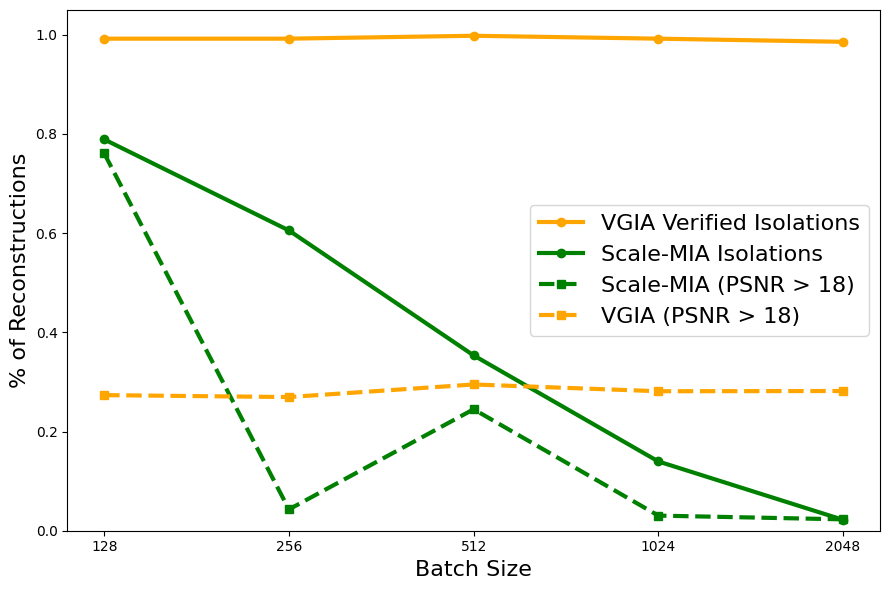
\includegraphics[width=0.32\linewidth]{assets/chapter_4/cifar/ratio_resnet.png}
    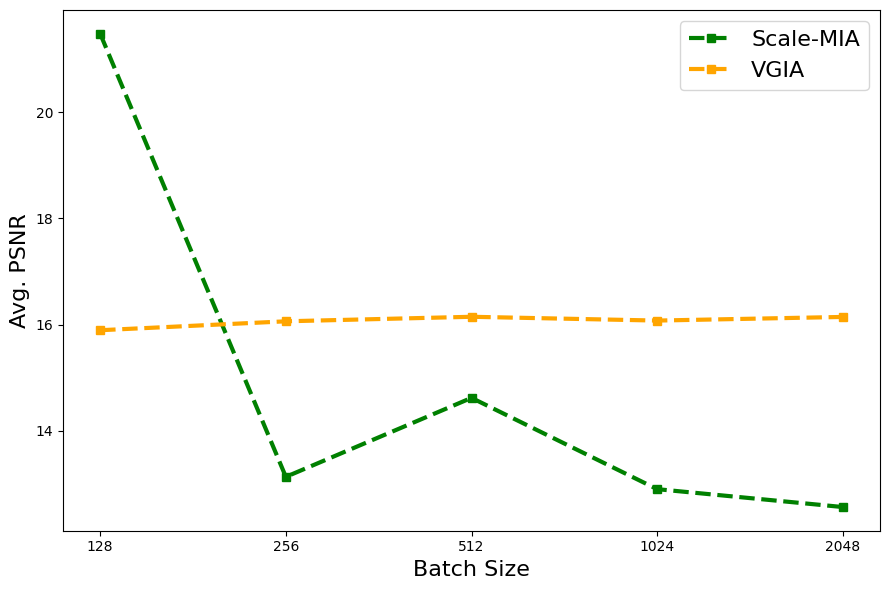
\includegraphics[width=0.32\linewidth]{assets/chapter_4/cifar/psnr_resnet.png}
    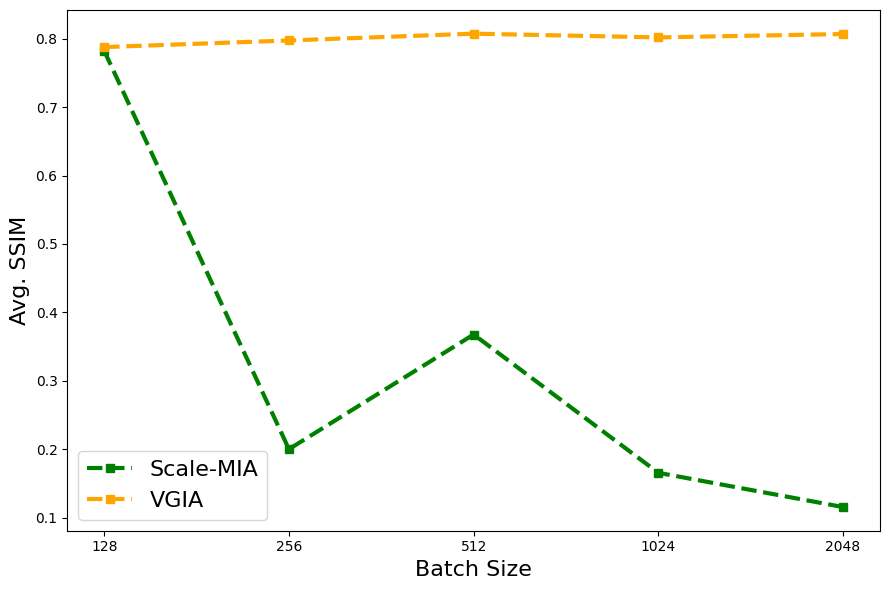
\includegraphics[width=0.32\linewidth]{assets/chapter_4/cifar/ssim_resnet.png}
    \caption{ResNet}
\end{subfigure}

\vspace{0.5em}

% --- Second row ---
\begin{subfigure}{\textwidth}
    \centering
    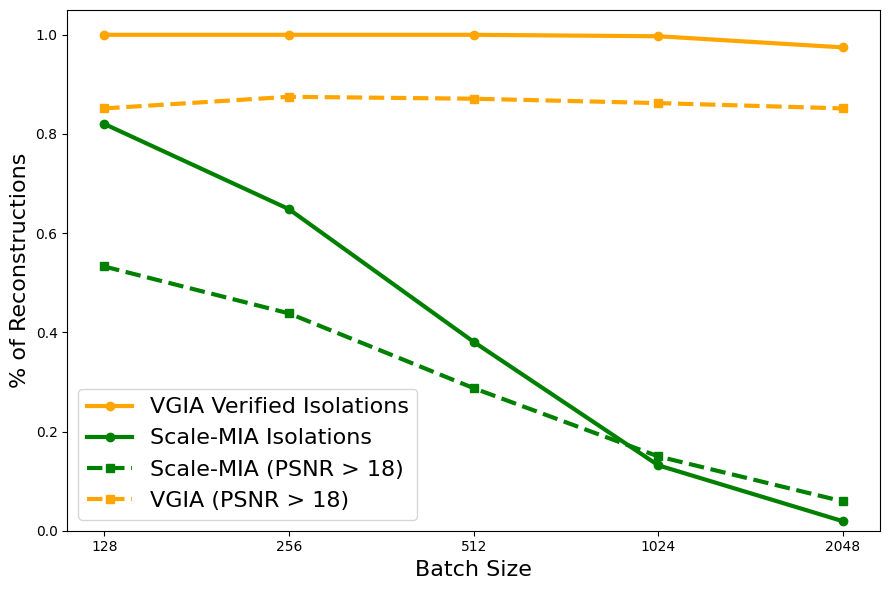
\includegraphics[width=0.32\linewidth]{assets/chapter_4/cifar/ratio_vit.png}
    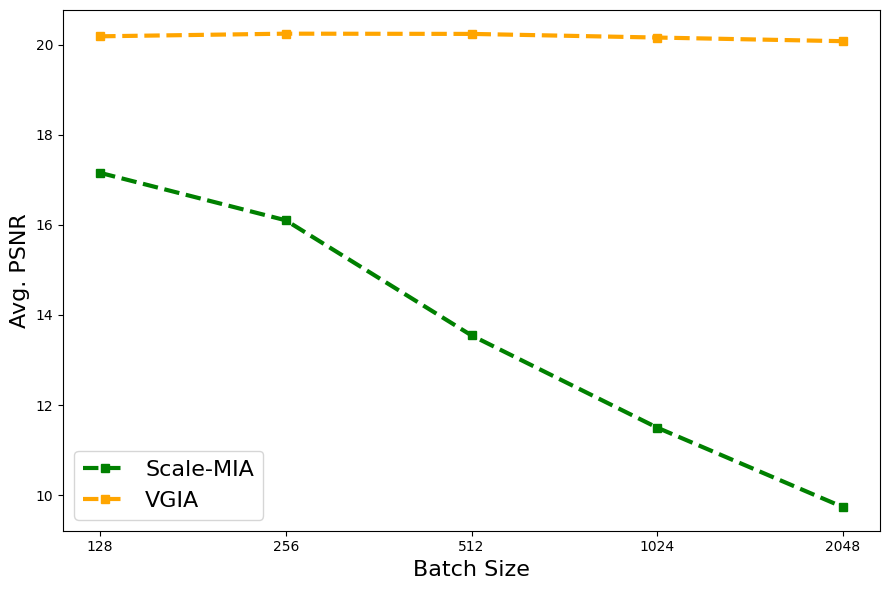
\includegraphics[width=0.32\linewidth]{assets/chapter_4/cifar/psnr_vit.png}
    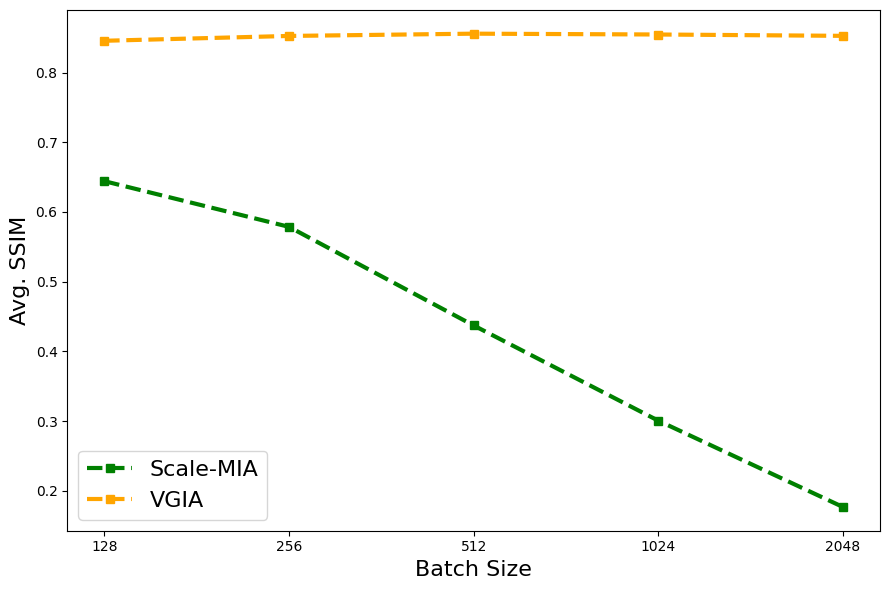
\includegraphics[width=0.32\linewidth]{assets/chapter_4/cifar/ssim_vit.png}
    \caption{ViT}
\end{subfigure}

\caption{Comparison of VGIA and Scale-MIA across different batch sizes. Each row corresponds to a model architecture, while columns report different evaluation metrics. From left to right: (i) percentage of correctly reconstructed samples (according to each method’s criterion), (ii) average PSNR of the decoded inputs, and (iii) average SSIM of the reconstructed samples. (a) Results on ResNet. (b) Results on ViT.}
\label{fig:vgia_scale_mia_results}
\end{figure}

\begin{figure*}
    \centering 
    % First row
    \subfloat[ResNet]{%
        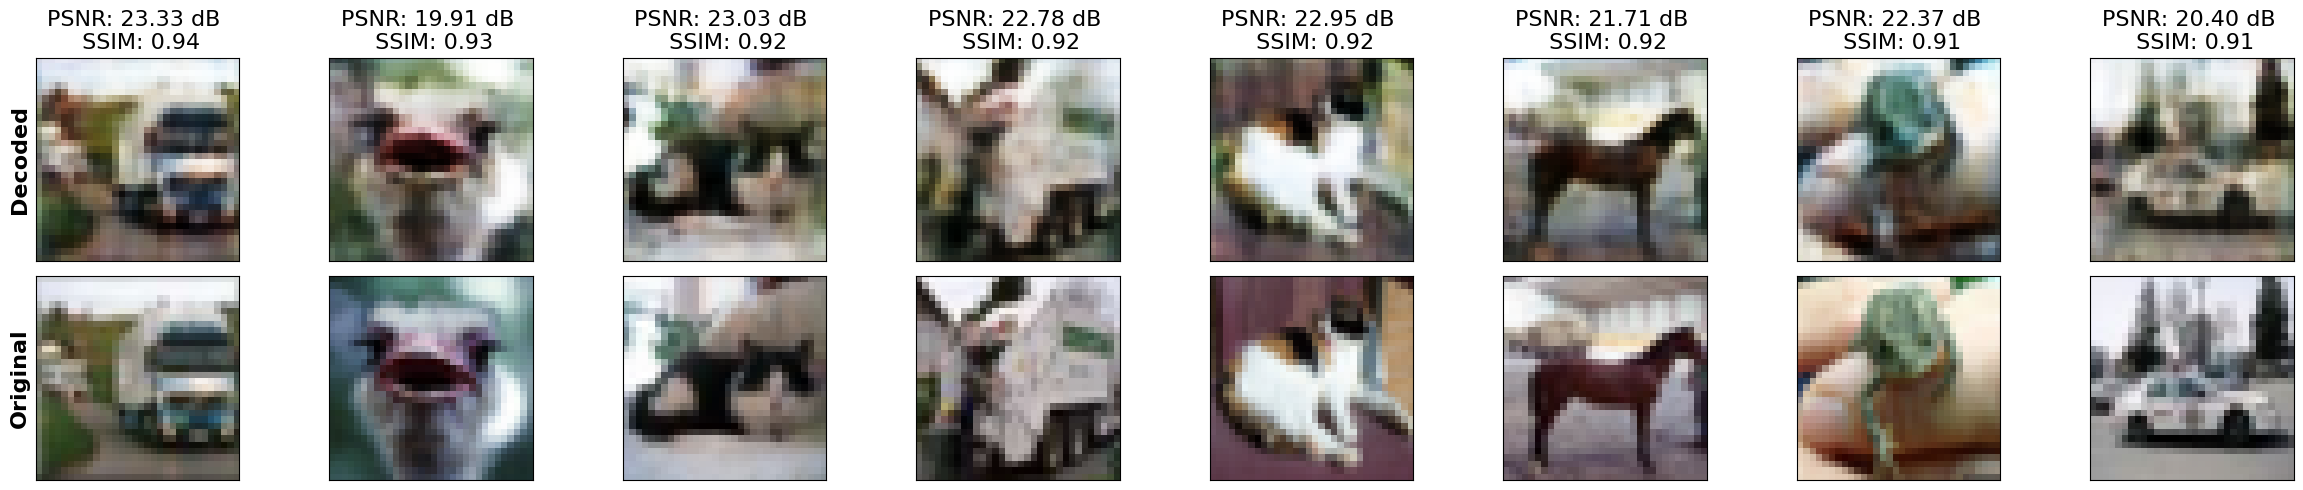
\includegraphics[width=1\linewidth]{assets/chapter_4/cifar/resnet_recon.png}
    }\\
    \subfloat[ViT ]{%
        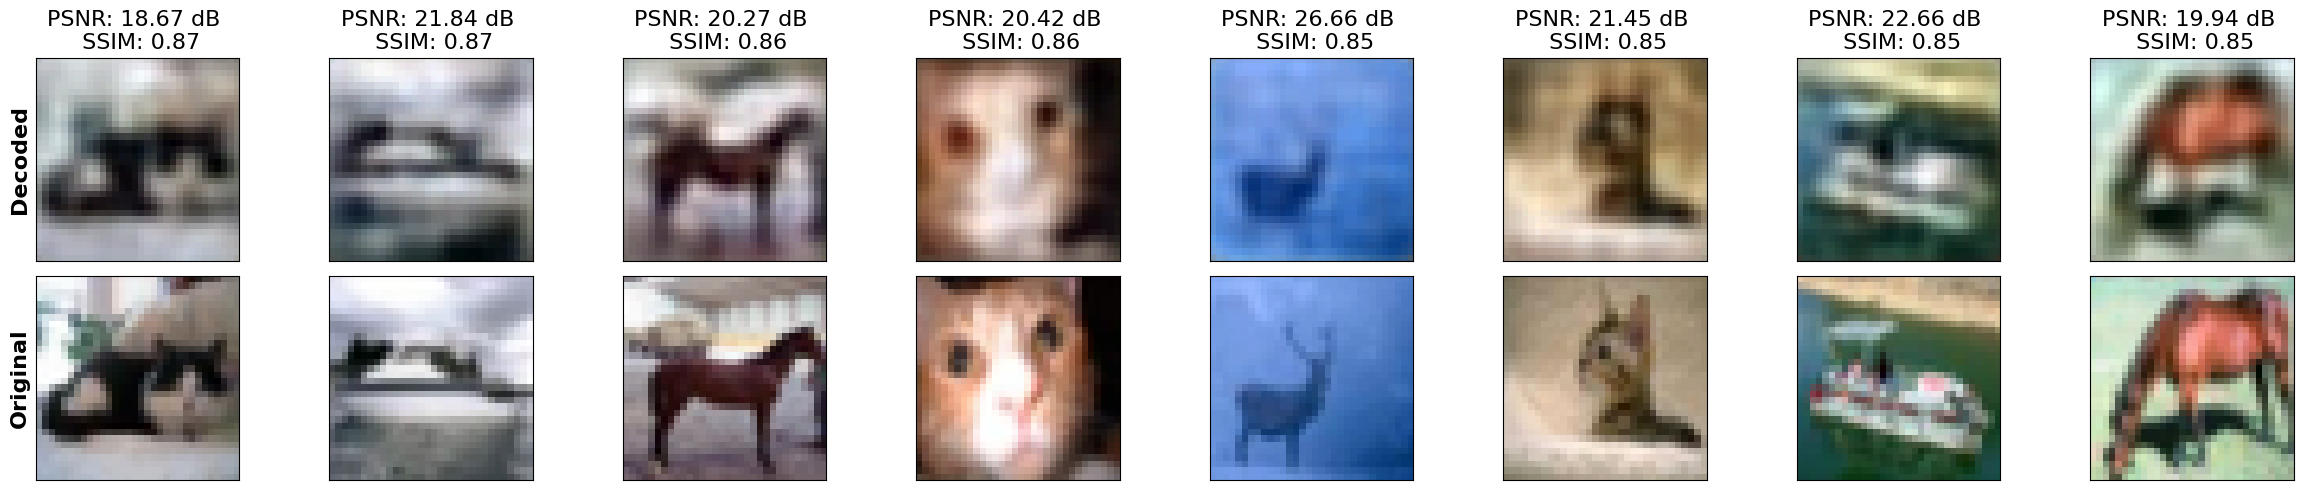
\includegraphics[width=1\linewidth]{assets/chapter_4/cifar/recon_vit.png}
    }\vspace{0.025\linewidth}
    \caption{Examples of reconstructed images from VGIA on a batch of $B=1024$ CIFAR10 samples. }
    \label{fig:rec_examples}
     \end{figure*}

\subsubsection{Results on Decepticons Attack}

\francesco{check if to keep it or not}
\subsection{Preliminary Defense Evaluation}\label{sec:vgia_defenses}

We conduct preliminary experiments to evaluate the robustness of our attack under common perturbation mechanisms, focusing on gradient clipping and additive Gaussian noise.

\subsubsection{Gradient Clipping}
Gradient clipping aims to bound the magnitude of gradient updates, potentially limiting the information available for reconstruction. However, from Eq.~\eqref{eq:hp_diff}, the effect of clipping can be written as\begin{equation}
    \frac{1}{B} \sum_{\substack{j \in \activeset_{i+1} \\ j \notin \activeset_{i}}} \gamma_j\frac{\partial \loss_j}{\partial z^{L}} \x_j  \quad \mathrm{where} \quad \gamma_j = \min(1,\; \frac{C}{\|\nabla_\theta \loss_j\|_2}).
\end{equation}
Thus, clipping only rescales individual sample contributions. As long as all gradients are clipped, the algebraic structure of the signal is preserved, and the verification condition in Prop.~\ref{prop:sample_isolation} remains valid without modification. In practice, an attacker can enforce this regime by increasing the magnitude of the model parameters, ensuring that all per-sample gradients are clipped. To validate this observation, we evaluate VGIA under different clipping thresholds on the ACS Income dataset with batch size $B=2048$. Results in Table~\ref{tab:clipping} show that the attack performance remains essentially unchanged across clipping levels, achieving near-perfect recovery in all settings.


\begin{table}[t]
\centering
\caption{Reconstruction performance under different clipping norms on the ACS Income dataset for $B=2048$.}

\begin{tabular}{lcc}
\toprule
Clipping Norm & \% Reconstructions & L2 Error \\
\midrule
10 & 99.90\% & $1.10 \times 10^{-25}$ \\
5  & 99.90\% & $1.10 \times 10^{-25}$ \\
2  & 99.80\% & $2.90 \times 10^{-26}$ \\
1  & 99.80\% & $2.90 \times 10^{-26}$ \\
\bottomrule
\end{tabular}
\label{tab:clipping}
\end{table}



\paragraph{Gradient Noise}
We also evaluate the behavior of our attack under Gaussian noise
perturbation. In this setting, the server observes noisy linear combinations
of the inputs. In particular, \eqref{eq:hp_diff} becomes
\begin{equation}
    \tilde{\mathbf{s}}_k =
    \frac{1}{B}
    \sum_{\substack{j \in \activeset_{i+1} \\ j \notin \activeset_i}}
    \frac{\partial \loss_j}{\partial z^L}\x_j
    + \frac{\eta_{i+1}}{g_{i+1}}-\frac{\eta_i}{g_i},
    \qquad
    \eta_i,\eta_{i+1}\sim\mathcal{N}(0,\sigma^2 I).
\end{equation}

Because of this noise, the exact span verification mechanism in
Prop.~\ref{prop:sample_isolation} cannot be applied. We instead use
thresholds to identify nonempty slices and to check whether a
previous-round slice is approximately in the span of its candidate
child slices. The attacker estimates the standard deviation $\sigma$ in
an initial calibration round. By placing the attack-layer hyperplanes
outside the known range of projected inputs, the attacker makes their
neurons inactive. Their clean weight gradients are therefore zero, and
the coordinates of the released weight gradients provide samples of
the added Gaussian noise.

Let $\hat\sigma$ be the estimated per-coordinate standard deviation
of this noise, and let $d$ be the input dimension. To identify a
nonempty slice, the implementation compares its norm with
\begin{equation}
    \tau_{\mathrm{empty}}
    = \hat\sigma\left(\sqrt{d}+\frac{1}{\sqrt{2}}\right).
\end{equation}
For span verification, we project the previous-round slice onto the
orthogonal complement of the subspace spanned by its candidate child
slices. If that subspace has rank $r$, we compare the residual norm with
\begin{equation}
    \tau_{\mathrm{span}}
    = \hat\sigma_{\mathrm{eff}}
      \left(\sqrt{d-r}+\frac{3}{\sqrt{2}}\right),
\end{equation}
where $\hat\sigma_{\mathrm{eff}}$ accounts for the scale factors of the
observations forming the previous-round slice. A residual below this
threshold is treated as consistent with the span relation. 
% %These are
% approximate checks, rather than the exact certificate available without
% noise. In particular, the empty-slice threshold used in these
% experiments does not adjust $\hat\sigma$ for the scaling of each slice.

We evaluate the attack on HARUS and CIFAR10 at different Gaussian
noise standard deviations. Figure~\ref{fig:noise_effect_vgia} shows
substantial recovery at the lower tested noise levels, followed by a
marked decrease as the noise increases. At the lowest tested standard
deviation, the attack produces approximately 584 and 779 correct
reconstructions, respectively, from batches of 1024 inputs using a
three-layer fully connected neural network with $N=1000$ attack
neurons.
\begin{figure*}
    \centering 
    \subfloat[HARUS]{%
        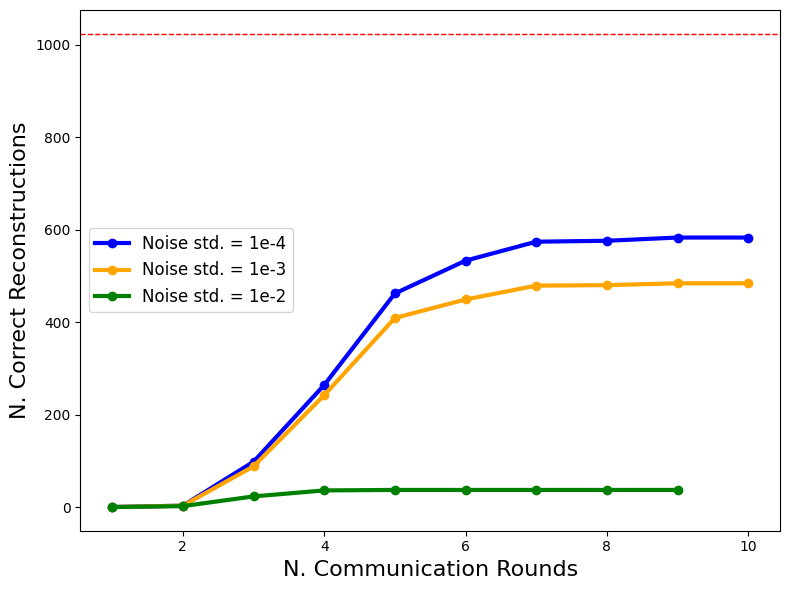
\includegraphics[width=0.45\linewidth]{assets/chapter_4/harus/noise_harus.png}
    }
    \subfloat[CIFAR10]{%
        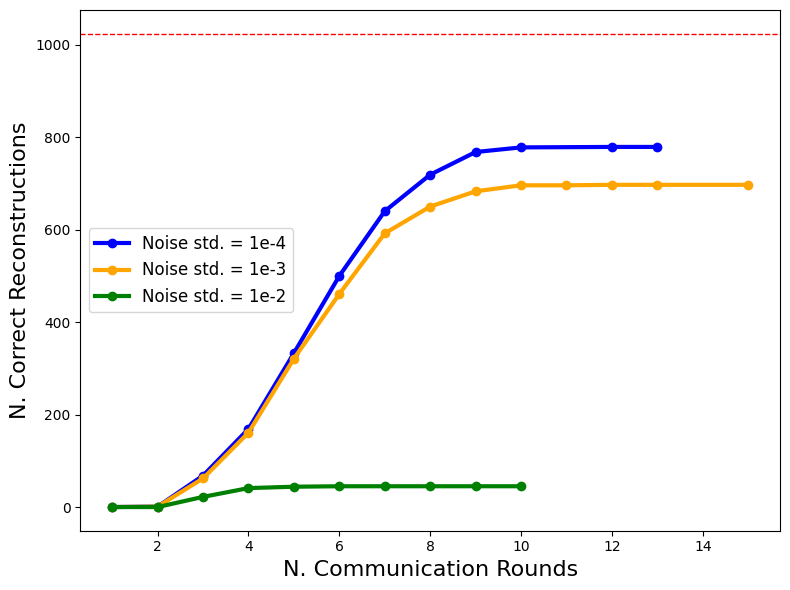
\includegraphics[width=0.45\linewidth]{assets/chapter_4/cifar/noise_cifar.png}
    }
    \vspace{0.025\linewidth}
    \caption{Number of reconstructed samples under increasing levels of Gaussian noise with variance $\sigma^2$. (a) Results on HARUS. (b) Results on CIFAR10.}
    \label{fig:noise_effect_vgia}
\end{figure*}

\section{Detectability of VGIA}
As discussed in Section~\ref{sec}, VGIA requires the attacker to configure the intermediate layers, from layer $a+1$ to layer $L-1$, so that the Jacobian entries $\frac{\partial z^L}{\partial z_i^a}$ are non-zero and independent of the input. When the inputs to these layers are non-negative, a simple way to satisfy this requirement is to assign positive weights and biases to all downstream layers, ensuring that every ReLU neuron remains active regardless of the input. We adopt this construction in the experiments presented in Section~\ref{sec:exp_main_vgia}.

However, the resulting parameter configurations may appear suspicious to clients that inspect the models received from the server before performing local training. To investigate the detectability of VGIA under less restrictive trust assumptions, we consider two alternative configurations designed to reduce the statistical evidence of malicious modifications while preserving the gradient structure required for reconstruction.

\subsection{Sampling from Realistic Distributions}

A first approach consists of constructing the intermediate layers, from layer $a+1$ to layer $L-1$, using parameters sampled from a zero-centered Gaussian distribution. The sampled values are assigned so that weights have relatively small magnitudes, while biases are preferentially selected from the tails of the distribution. When the sampled bias values are insufficient to enforce the desired activation pattern, the corresponding biases are instead chosen deterministically and may therefore fall outside the sampled distribution.

The attacker configures the parameters so that approximately half of the neurons in each intermediate layer remain permanently active and the other half permanently inactive, independently of the input. The resulting fixed activation pattern preserves the input-independent Jacobian required by VGIA while avoiding the uniformly positive weights and biases used in the original construction. Since the attacker knows the bounds on the input features, it can verify the activation pattern by propagating bounds through the network and checking that each pre-activation maintains the desired sign over the entire input domain.

We empirically validate this initialization strategy on the ACS Income dataset. Figure~\ref{fig:weight_dist} shows that the resulting malicious parameters still follow an approximately zero-mean Gaussian distribution, while Fig.~\ref{fig:vgia_gaussian_weight} shows that this initialization strategy does not affect the reconstruction performance of VGIA.


\begin{figure*}
    \centering 
    \subfloat[\label{fig:weight_dist}]{%
        \includegraphics[width=0.45\linewidth]{assets/chapter_4/income_california/weight_dist.pdf}
    }
    \subfloat[\label{fig:vgia_gaussian_weight}]{%
        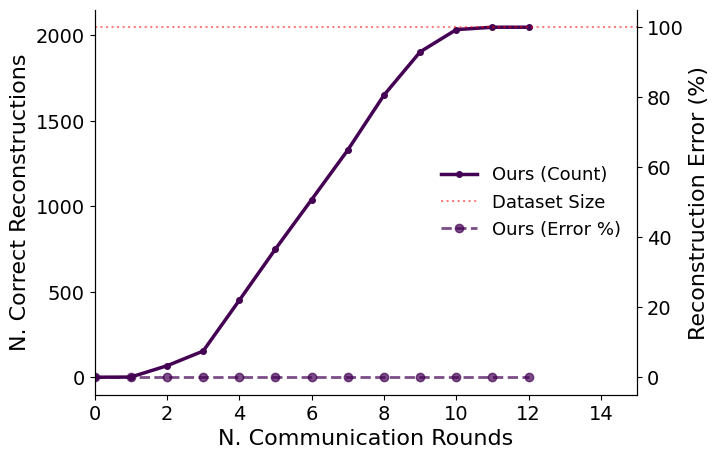
\includegraphics[width=0.45\linewidth]{assets/chapter_4/income_california/vgia_gaussian_weights.png}
    }
    \vspace{0.025\linewidth}
\caption{(a) Distribution of malicious parameters initialized from $\mathcal{N}(0,1)$. (b) VGIA performance on the ACS Income dataset with a batch size of 2048 under Gaussian parameter initialization.}
\end{figure*}

\subsection{Attacking a Subset of the Parameters}\label{sec:detectability}

In the experiments presented in Section~\ref{sec:exp_main_vgia}, the server assigns a search hyperplane to every neuron in the attacked layer. Consequently, all neurons share the same weight vector and differ only in their biases, introducing a highly structured parameter configuration that may be easily detected by a client inspecting the received model. To reduce the extent of these modifications, we consider a variant of VGIA that targets only a subset $\mathcal{P}$ of the $N$ neurons in layer $a$, with $N_a = |\mathcal{P}| < N$. For each attacked neuron $i\in\mathcal{P}$, the server sets $\W_i^a=\mathbf{w}$, where $\mathbf{w}\in\real^d$ is shared across the attacked neurons, and adjusts the corresponding bias according to Algorithm~\ref{algo:parallelattack}. The remaining neurons retain their parameters and continue to evolve through ordinary training updates.

As discussed in Section~\ref{sec:fedavg_vgia}, the gradient contributions of the attacked neurons can be factorized by routing their downstream influence through a carrier neuron. In that construction, the server establishes an isolated path through the subsequent hidden layers, disconnecting the carrier neurons from the rest of the network. For the purpose of reducing detectability, we consider a less restrictive construction that modifies only the connections between layers $a$ and $a+1$, while allowing the remaining downstream layers to retain their original parameters.

Let layer $a+1$ contain $M$ neurons, with $\W^{a+1}\in\real^{M\times N}$. The server selects a carrier neuron $\kappa$ and assigns nonzero connections from each attacked neuron to the carrier, while removing the connections from non-attacked neurons:
\begin{equation*}
W^{a+1}_{\kappa,i}
\begin{cases}
\neq 0, & i\in\mathcal P,\\
=0, & i\notin\mathcal P.
\end{cases}
\end{equation*}
As in the FedAvg construction, the carrier bias is chosen so that its pre-activation remains strictly positive over the admissible input domain. The carrier therefore operates in the linear regime of the ReLU activation for every possible input.

The connections from the attacked neurons to the remaining neurons of layer $a+1$ can be configured in two ways. The first follows the isolated-carrier construction introduced for FedAvg, setting $W^{a+1}_{r,i}=0$ for every $r\neq\kappa$ and $i\in\mathcal P$. Although this preserves the required gradient factorization, it introduces many zero-valued parameters that may facilitate detection.

To avoid these zero connections, we consider a second construction in which the corresponding weights are proportional to the carrier connections. Specifically, for each non-carrier neuron $r\neq\kappa$, the server selects a scalar $\lambda_r$ and sets
\begin{equation}
W^{a+1}_{r,i}
=
\lambda_r W^{a+1}_{\kappa,i},
\qquad \forall i\in\mathcal P.
\label{eq:stealth_proportional}
\end{equation}
The isolated-carrier construction corresponds to the special case $\lambda_r=0$ for every $r\neq\kappa$.

Under this configuration, the downstream Jacobian associated with an attacked neuron $i\in\mathcal P$ becomes
\begin{equation}
\frac{\partial z^L}{\partial z_i^a}
=
W^{a+1}_{\kappa,i}
\left[
\frac{\partial z^L}{\partial z_\kappa^{a+1}}
+
\sum_{\substack{r=1\\r\neq\kappa}}^M
\lambda_r
\indicator_{\{z_r^{a+1}>0\}}
\frac{\partial z^L}{\partial z_r^{a+1}}
\right].
\label{eq:stealth_jacobian}
\end{equation}
Although the terms inside the brackets may depend on the input and on the activation patterns of subsequent layers, they are shared across all attacked neurons. Consequently, for each sample $(\x_j,y_j)$, we can define the sample-dependent coefficient
\begin{equation}
\rho_j
=
\left.
\left[
\frac{\partial\mathcal L_j}{\partial z^L}
\left(
\frac{\partial z^L}{\partial z_\kappa^{a+1}}
+
\sum_{\substack{r=1\\r\neq\kappa}}^M
\lambda_r
\indicator_{\{z_r^{a+1}>0\}}
\frac{\partial z^L}{\partial z_r^{a+1}}
\right)
\right]\right|_{\x=\x_j},
\end{equation}
which is independent of the attacked-neuron index $i$. The gradient therefore factorizes as
\begin{equation}
\frac{\partial\mathcal L_j}{\partial z_i^a}
=
W^{a+1}_{\kappa,i}\rho_j.
\label{eq:stealth_factorization}
\end{equation}

The resulting factorization has the same structure as the one derived for the FedAvg carrier construction. Hence, normalizing the weight and bias gradients of each attacked neuron by the corresponding coefficient $W^{a+1}_{\kappa,i}$ allows the server to recover the slice vectors $\slice_k$ and $\beta_k$ through the same gradient-difference procedure. In particular, the contributions of samples activating two consecutive attacked neurons cancel exactly, as in Eq.~\eqref{eq:hp_diff}. When a slice contains a single sample $\x_j$ with $\rho_j\neq 0$, its input can therefore be reconstructed exactly from $\slice_k/\beta_k$.

Unlike the isolated carrier path introduced for FedAvg, the proportional construction requires no modifications beyond layer $a+1$ and does not constrain the activation patterns of the remaining downstream neurons. It also applies to both regression and multiclass classification without requiring the classification-layer modifications described in Section~\ref{sec:multiclass_vgia}.

However, the additional flexibility introduces two potential limitations. First, contributions propagated through different downstream neurons may cancel, yielding $\rho_j=0$ for some samples and preventing their reconstruction. Second, the construction does not guarantee that the coefficients associated with different samples satisfy the conditions required by Proposition~\ref{prop:sample_isolation} across communication rounds. Consequently, the theoretical verification guarantees do not necessarily extend to this setting.

Nevertheless, in our experiments, we did not observe zero coefficients, verification failures attributable to the modified construction, or measurable degradation in reconstruction performance.

\subsection{Perturb Attack Directions}

Restricting the attack to the neurons in $\mathcal P$ reduces the number of
modified rows, and consequently, the imprint of the attack in the model parameters. However, assigning the same direction $\w$ to all attacked
neurons still introduces a repeated structure in the attacked layer. To reduce
this regularity, the server can apply a small, independent perturbation to the
direction of each attacked neuron. This modification affects only the weight
vectors of the attacked neurons, while the proportional connections introduced
above remain unchanged.

At each attack round $t$, and for each attacked neuron $i\in\mathcal P$, the
server samples
\begin{equation*}
    \boldsymbol{\xi}_i
    \sim
    \mathcal N(\mathbf 0,\mathbf I_d),
\end{equation*}
and projects it onto the subspace orthogonal to the reference attack direction
$\w$. Let
\begin{equation*}
    \widehat{\w}
    =
    \frac{\w}{\|\w\|}
\end{equation*}
denote the normalized attack direction. The orthogonal component is
\begin{equation*}
    \boldsymbol{\xi}^{\perp}_i
    =
    \boldsymbol{\xi}_i
    -
    \left(
        \boldsymbol{\xi}_i^\top
        \widehat{\w}
    \right)
    \widehat{\w}.
\end{equation*}
The server then normalizes this component as
\begin{equation*}
    \widehat{\boldsymbol{\xi}}^{\perp}_i
    =
    \frac{
         \boldsymbol{\xi}^{\perp}_i
    }{
        \left\|
             \boldsymbol{\xi}^{\perp}_i
        \right\|
    }.
\end{equation*}

Given a perturbation parameter $p\geq 0$, the server sets the weight vector of each attacked neuron $i\in\mathcal P$ to
\begin{equation}
\label{eq:perturbed_direction}
\W_i^{a}
=
\|\w\|
\frac{
\widehat{\w}
+
p \mathbf{\widehat{\boldsymbol{\xi}}^{\perp}_i}
}{
\sqrt{1+p^2}
}.
\end{equation}
The parameter $p$ controls the magnitude of the orthogonal perturbation relative to the reference direction. Since
$\widehat{\boldsymbol{\xi}}^{\perp \top}_i\widehat{\w}=0$ and $\|\widehat{\boldsymbol{\xi}}^{\perp}_i\|=1$, the construction preserves the norm of the original attack direction, and its cosine similarity with $\w$ is
\begin{equation*}
\frac{
\left(\W_i^{a}\right)^\top\w
}{
\left\|\W_i^{a}\right\|
\|\w\|
}
=
\frac{1}{\sqrt{1+p^2}}.
\end{equation*}
Hence, the angle between each perturbed direction and the reference direction $\w$ is $\arctan(p)$. The weights of neurons outside $\mathcal P$ are left unchanged.

For $p>0$, however, the hyperplanes associated with the attacked neurons are no longer exactly parallel. Consequently, the active sets $\mathcal A_i$ and $\mathcal A_{i'}$ associated with two consecutive queried neurons are no longer guaranteed to be nested. Their normalized gradient difference becomes
\begin{equation*}
\frac{1}{B}
\sum_{j\in\mathcal A_{i'}\setminus\mathcal A_i}
\rho_j\x_j
-
\frac{1}{B}
\sum_{j\in\mathcal A_i\setminus\mathcal A_{i'}}
\rho_j\x_j,
\end{equation*}
instead of the single set difference appearing in
Eq.~\eqref{eq:stealth_slice}. In the parallel case, nesting of the active sets guarantees that the second term vanishes, but under direction perturbation, this property is no longer guaranteed. The VGIA search continues to select the bias values with respect to the reference direction $\w$. However, the perturbed hyperplanes can induce active sets that differ from those implied by the reference search, so the regions
identified during the search do not necessarily coincide with the regions
defined by the perturbed neurons. Since the perturbations are independently
resampled across communication rounds, this mismatch can vary over time.
As a result, reconstruction performance may degrade as the perturbation
magnitude $p$ increases. We evaluate this trade-off empirically for different
values of $p$.

\subsection{Experiments for Stealthier Attacks}
\label{app:exp_stealthier_attack}
We evaluate the impact of the proposed modifications on both the reconstruction
performance and detectability of VGIA. We first study the effect of perturbing
the attack directions on reconstruction performance. We then assess
detectability through hypothesis testing, evaluating whether state-of-the-art
metrics for detecting active gradient inversion attacks~\cite{carletti2026detectability}
can distinguish attacked models from benign ones.

\subsubsection{Effect of perturbation}
We evaluate different values of the perturbation parameter $p$, with the
results reported in Figure~\ref{fig:perturbation_results}. As expected,
reconstruction performance gradually decreases as the perturbation magnitude
increases. On ACS Income, the fraction of correctly reconstructed samples decreases
from $100\%$ for $p=0$ to $98\%$ for $p=10^{-6}$ and $66\%$ for
$p=10^{-4}$. Similarly, on CIFAR-10, it decreases from $100\%$ for $p=0$
to $88\%$ for $p=10^{-6}$ and $53\%$ for $p=10^{-4}$. We observe a
similar trend across the remaining datasets.

Importantly, even very small perturbations are sufficient to eliminate thex
rank deficiency induced by the original parallel construction, yielding a
full-rank attacked weight matrix.

\begin{figure}
    \centering
    \includegraphics[width=0.6\linewidth]{assets/chapter_4/iclr_version/vgia_perturbation_crr.pdf}
\caption{Percentage of correct reconstructions for increasing values of the direction perturbation $p$. Lines show the mean over three random seeds, and shaded regions show one standard deviation. We use \(B=2048\) for all datasets except ImageNet, for which \(B=1024\). Each client computes one full-batch FedSGD gradient per communication round.}    \label{fig:perturbation_results}
\end{figure}

We next assess whether monitoring the client's training loss is sufficient to
detect the attack. We set $N_a=100$ and let the server retain the
client-updated values of all non-attacked parameters across communication
rounds, modifying only the parameters required by the attack. As shown in
Table~\ref{tab:training_loss_crr}, with
$p=10^{-7}$ and a fixed budget of $90$ communication rounds, VGIA recovers
nearly the entire client dataset with negligible reconstruction error while
maintaining a full-rank attacked weight matrix. At the same time, the training
loss continues to decrease during training, showing that loss monitoring alone
does not provide a reliable indicator of the attack.

\begin{table}[t]
    \centering
    \small
    \caption{Training loss and VGIA correct reconstruction rate across communication rounds. Each cell reports the training loss (top) and the percentage of correct reconstructions (bottom), as mean $\pm$ standard deviation over three random seeds. The attacker uses $N_a=100$ neurons. Each dataset has $B=2048$ samples, except for ImageNet, for which $B=1024$.}
    \label{tab:training_loss_crr}

    \setlength{\tabcolsep}{5pt}
    \renewcommand{\arraystretch}{1.08}

    \resizebox{\linewidth}{!}{%
    \begin{tabular}{@{}cccccc@{}}
        \toprule
        \textbf{Round}
        & \textbf{ACS Income}
        & \textbf{King County Housing}
        & \textbf{HARUS}
        & \textbf{CIFAR-10}
        & \textbf{ImageNet} \\
        \midrule

        10
        & \shortstack{$(8.06\pm9.87)\!\times\!10^{-1}$\\ $9.93\pm0.40$}
        & \shortstack{$1.06\pm0.02$\\ $10.3\pm0.45$}
        & \shortstack{$1.93\pm0.05$\\ $10.2\pm0.78$}
        & \shortstack{$2.61\pm0.06$\\ $9.72\pm0.51$}
        & \shortstack{$12.9\pm0.78$\\ $20.8\pm0.64$} \\

        \addlinespace[0.35em]
        20
        & \shortstack{$(4.27\pm4.96)\!\times\!10^{-1}$\\ $22.0\pm0.57$}
        & \shortstack{$1.03\pm0.03$\\ $22.2\pm0.16$}
        & \shortstack{$1.80\pm0.05$\\ $22.9\pm0.60$}
        & \shortstack{$2.48\pm0.03$\\ $22.4\pm0.38$}
        & \shortstack{$12.7\pm0.77$\\ $45.4\pm1.42$} \\

        \addlinespace[0.35em]
        30
        & \shortstack{$(1.89\pm1.79)\!\times\!10^{-1}$\\ $34.6\pm1.15$}
        & \shortstack{$1.02\pm0.03$\\ $34.3\pm0.71$}
        & \shortstack{$1.71\pm0.09$\\ $34.8\pm0.50$}
        & \shortstack{$2.38\pm0.04$\\ $34.8\pm0.50$}
        & \shortstack{$12.5\pm0.76$\\ $70.7\pm3.20$} \\

        \addlinespace[0.35em]
        40
        & \shortstack{$(7.46\pm3.76)\!\times\!10^{-2}$\\ $47.5\pm0.77$}
        & \shortstack{$1.00\pm0.03$\\ $46.7\pm0.66$}
        & \shortstack{$1.65\pm0.10$\\ $47.1\pm0.52$}
        & \shortstack{$2.34\pm0.03$\\ $46.7\pm0.57$}
        & \shortstack{$12.1\pm0.73$\\ $96.6\pm3.57$} \\

        \addlinespace[0.35em]
        50
        & \shortstack{$(3.65\pm0.72)\!\times\!10^{-2}$\\ $59.9\pm0.59$}
        & \shortstack{$(9.82\pm0.34)\!\times\!10^{-1}$\\ $58.6\pm1.31$}
        & \shortstack{$1.61\pm0.10$\\ $59.6\pm0.83$}
        & \shortstack{$2.31\pm0.02$\\ $58.8\pm1.07$}
        & \shortstack{$12.1\pm0.73$\\ $99.9\pm0.10$} \\

        \addlinespace[0.35em]
        60
        & \shortstack{$(2.54\pm0.52)\!\times\!10^{-2}$\\ $72.0\pm0.76$}
        & \shortstack{$(9.63\pm0.38)\!\times\!10^{-1}$\\ $71.1\pm1.58$}
        & \shortstack{$1.56\pm0.09$\\ $71.9\pm0.20$}
        & \shortstack{$2.30\pm0.02$\\ $71.1\pm0.81$}
        & -- \\

        \addlinespace[0.35em]
        70
        & \shortstack{$(2.14\pm0.29)\!\times\!10^{-2}$\\ $84.4\pm0.59$}
        & \shortstack{$(9.43\pm0.41)\!\times\!10^{-1}$\\ $84.0\pm1.98$}
        & \shortstack{$1.51\pm0.07$\\ $84.5\pm0.93$}
        & \shortstack{$2.30\pm0.02$\\ $83.9\pm0.73$}
        & -- \\

        \addlinespace[0.35em]
        80
        & \shortstack{$(1.98\pm0.16)\!\times\!10^{-2}$\\ $97.7\pm1.26$}
        & \shortstack{$(9.21\pm0.45)\!\times\!10^{-1}$\\ $96.8\pm2.74$}
        & \shortstack{$1.46\pm0.06$\\ $98.0\pm1.39$}
        & \shortstack{$2.29\pm0.02$\\ $96.5\pm0.99$}
        & -- \\

        \addlinespace[0.35em]
        90
        & \shortstack{$(1.78\pm0.09)\!\times\!10^{-2}$\\ $99.8\pm0.03$}
        & \shortstack{$(9.24\pm0.36)\!\times\!10^{-1}$\\ $99.6\pm0.18$}
        & \shortstack{$1.45\pm0.05$\\ $99.8\pm0.06$}
        & \shortstack{$2.29\pm0.02$\\ $99.8\pm0.10$}
        & -- \\

        \bottomrule
    \end{tabular}
    }
\end{table}


\subsubsection{Detectability metrics}

We evaluate the detectability of VGIA using the statistical metrics proposed by~\citeA{carletti2026detectability}, which examine the rank of the weight matrix, the variability of neuron weight vectors, the entropy of quantized weight values, the ordering of neuron biases, and the differences between consecutive biases. VGIA can mitigate the last two detection criteria by assigning biases to arbitrary neuron indices and rescaling the weight vector and bias of each attacked neuron by the same positive factor, thereby preserving the corresponding hyperplane. We therefore focus on matrix rank, neuron variability, and weight entropy.

We additionally investigate the mean weight value and the mean pairwise cosine similarity between neuron weight vectors. While most of these statistics characterize the model received at an individual communication round, a client may also retain and compare successive models to identify suspicious patterns across training. We consequently evaluate cosine similarity both within individual rounds and cumulatively over multiple communication rounds. Finally, we consider a simple loss-based sanity check that examines whether the training loss decreases over successive rounds.

We formulate the detection problem as a binary hypothesis test, distinguishing between models generated by benign training and models modified by a malicious server:
\begin{equation*}
\begin{aligned}
H_0 &: \quad \text{The received model follows the prescribed training procedure},\\
H_1 &: \quad \text{The received model has been maliciously modified by the server}.
\end{aligned}
\end{equation*}
For each detection statistic, we estimate its empirical distribution under $H_0$ by training $100$ benign models on the Income dataset for $100$ communication rounds, using standard PyTorch Kaiming initialization. We compute the corresponding statistics at each training checkpoint and use the resulting observations to characterize benign behavior.

We define the acceptance region of each test as the central $95\%$ interval of the corresponding empirical null distribution, yielding a nominal false-positive rate (FPR) of $5\%$. A model is classified as suspicious when its detection statistic falls outside this interval. We then report the false-negative rate (FNR), defined as the fraction of attacked models whose statistics remain within the acceptance region. For the cross-round experiments, the null distribution is calibrated using the corresponding statistics computed over benign training trajectories.

Unless otherwise specified, we consider $N_a=10$ attacked neurons and a perturbation magnitude of $p=10^{-7}$. The reference attack direction $\w$ is sampled using Kaiming initialization, and the attacked neurons are perturbed according to Equation~\eqref{eq:perturbed_direction}.

We also investigate a variant that uses two opposite reference directions, $\w$ and $-\w$. In particular, the server constructs perturbed weight vectors around $\w$ for
\begin{equation*}
N_a' \approx \frac{N_a+\sqrt{N_a}}{2}
\end{equation*}
attacked neurons, and around $-\w$ for the remaining $N_a-N_a'$ neurons. The allocation approximately balances the positive and negative contributions of the attacked vectors to the average pairwise inner product, reducing the statistical signal associated with their common direction.


\subsubsection{Rank-based detection} We first examine whether direction perturbations can eliminate the rank deficiency introduced by the parallel-hyperplane construction. As shown in Figure~\ref{fig:perturbation_results}, reconstruction performance gradually decreases as the perturbation magnitude increases. In particular, for $p=10^{-7}$, VGIA reconstructs more than $95\%$ of the samples on every dataset while maintaining a full-rank weight matrix. Thus, even a very small direction perturbation removes the rank deficiency of the parallel construction with only a limited impact on reconstruction performance.

\subsubsection{Single-round detection}

We next examine whether the remaining parameter statistics can distinguish benign and attacked models at individual communication rounds.

Table~\ref{tab:single_round_variability_entropy} reports the results for weight variability and quantized-weight entropy. With a single attack direction, the two metrics yield FNRs of $88.16\%$ and $95.16\%$, respectively, indicating limited ability to distinguish attacked models from those obtained through benign training. The use of two opposite directions further increases the FNR of the weight-variability detector to $91.07\%$, while the entropy detector remains essentially unaffected, with an FNR of $95.05\%$. For weight entropy, the resulting detection rate is approximately $5\%$, close to the nominal FPR, suggesting little separation between the benign and attacked distributions under this statistic.

% We then evaluate the detection metrics proposed by~\citeA{carletti2026detectability}. These metrics examine the rank of the weight matrix, the variability of the neuron weight vectors, the entropy of the quantized weight values, the ordering of the neuron biases, and the differences between consecutive biases. VGIA can directly avoid the last two tests. The server can assign the biases to arbitrary neuron indices and can scale the weight vector and bias of each attacked neuron by the same factor without changing its hyperplane. We therefore evaluate the matrix rank, neuron variability, and weight entropy. As shown in Figure~\ref{fig:perturbation_results}, reconstruction performance gradually decreases as the perturbation magnitude increases. In particular, for $p=10^{-7}$, VGIA reconstructs more than $95\%$ of the samples on every dataset while maintaining a full-rank weight matrix. Thus, even a very small direction perturbation removes the rank deficiency of the parallel construction with only a limited impact on reconstruction performance.


% We evaluate the cosine-similarity test both within individual communication rounds and over the complete training trajectory, since a client must monitor all the models received during training. Finally, we consider a simple sanity check where a client just tests if the training loss is decreasing across training rounds.

% The attacked weight matrix has a rank ratio equal to one for all tested perturbation levels and datasets. 
% %In particular, for $p=10^{-7}$, VGIA reconstructs more than $95\%$ of the samples on every dataset, while the attacked weight matrix remains full rank. Thus, even a very small direction perturbation removes the rank deficiency of the parallel construction with only a limited impact on reconstruction performance. 
% As shown in Fig.~\ref{fig:perturbation_results}, reconstruction performance gradually decreases as the perturbation magnitude increases. In particular, for $p=10^{-7}$, VGIA reconstructs more than $95\%$ of the
% samples on every dataset while maintaining a full-rank weight matrix. Thus, even a very small direction perturbation removes the rank deficiency of the parallel construction with only a limited impact on reconstruction performance.


% In addition to the metrics of~\citeA{carletti2026detectability}, we consider the mean
% weight value and the mean pairwise cosine similarity between neuron weight
% vectors. We evaluate cosine similarity both within each communication round
% and cumulatively across the training trajectory, since a client may retain and
% compare the sequence of models received throughout training. Finally, we
% consider a simple loss-based sanity check that tests whether the training loss
% decreases over successive communication rounds.

% We evaluate these metrics using hypothesis tests. For each detection statistic,
% the null hypothesis corresponds to the behavior observed under benign
% training. We estimate its empirical null distribution by training $100$
% benign models on the Income dataset for $100$ communication rounds using
% standard PyTorch Kaiming initialization and computing the corresponding
% detection statistics at each checkpoint. We define the acceptance region as
% the central $95\%$ interval of the empirical benign distribution, yielding a
% target false-positive rate (FPR) of $5\%$, and report the resulting
% false-negative rate (FNR) on attacked models.

% For the attacked models, we set $N_a=10$ attacked neurons and evaluate each
% training checkpoint using the same detection procedure. The reference attack
% direction $\w$ is sampled using Kaiming initialization and perturbed with
% $p=10^{-7}$. We additionally evaluate a variant of VGIA that uses two
% opposite reference directions, $\w$ and $-\w$. Specifically, the server
% constructs perturbed vectors around $\w$ for
% \begin{equation*}
% N_a' \approx \frac{N_a+\sqrt{N_a}}{2}
% \end{equation*}
% attacked neurons and around $-\w$ for the remaining $N_a-N_a'$ neurons.
% This allocation approximately balances the positive and negative
% contributions of the attacked vectors to the average pairwise inner product,
% thereby reducing the signal exposed by pairwise-similarity statistics.


% Table~\ref{tab:single_round_variability_entropy} reports the statistics
% obtained from the empirical benign distribution and the attacked models,
% together with the corresponding FNR. With a single attack direction, weight variability yields an FNR of $88.16\%$, while weight entropy yields an FNR of $95.16\%$. These results indicate that both statistics provide limited separation between benign and attacked models when evaluated on weights obtained from actual training. Using two independently perturbed opposite directions further increases the
% FNR of the weight-variability detector to $91.07\%$. Weight entropy remains
% essentially unaffected, with an FNR of $95.05\%$. In the latter case, the
% corresponding detection rate is approximately $5\%$, close to the nominal
% $5\%$ FPR, indicating almost no separation between the benign and attacked
% distributions.

\begin{table*}[t]
\centering
\caption{Single-round detection results for weight variability and quantized-weight entropy. For each metric, we report the mean $\pm$ standard deviation for benign and attacked models, the central $95\%$ interval of the empirical benign distribution, and the resulting false-negative rate (FNR). Results are shown for VGIA with one reference direction and with two opposite reference directions, using $N_a=10$ attacked neurons and perturbation magnitude $p=10^{-7}$.}
\label{tab:single_round_variability_entropy}
\resizebox{\textwidth}{!}{%
\begin{tabular}{lccccc}
\toprule
Metric
& No. of directions
& Benign mean \(\pm\) std
& Benign \(95\%\) interval
& Attacked mean \(\pm\) std
& FNR (\%) \\
\midrule
Weight variability
& \(1\)
& \(8.16\times10^{-1} \pm 3.60\times10^{-4}\)
& \([8.16\times10^{-1},\,8.17\times10^{-1}]\)
& \(8.16\times10^{-1} \pm 3.77\times10^{-4}\)
& \(88.16\) \\

Weight variability
& \(2\)
& \(8.16\times10^{-1} \pm 3.60\times10^{-4}\)
& \([8.16\times10^{-1},\,8.17\times10^{-1}]\)
& \(8.16\times10^{-1} \pm 3.76\times10^{-4}\)
& \(91.07\) \\

Weight entropy
& \(1\)
& \(3.31 \pm 1.40\times10^{-2}\)
& \([3.27,\,3.32]\)
& \(3.31 \pm 1.39\times10^{-2}\)
& \(95.16\) \\

Weight entropy
& \(2\)
& \(3.31 \pm 1.40\times10^{-2}\)
& \([3.27,\,3.32]\)
& \(3.31 \pm 1.39\times10^{-2}\)
& \(95.05\) \\
\bottomrule
\end{tabular}%
}
\end{table*}

We then consider the mean pairwise cosine similarity between neuron weight vectors. Unlike variability and entropy, cosine similarity directly captures the directional structure introduced by the attack. As shown in Table~\ref{tab:cumulative_cosine_single}, the single-direction construction yields an FNR of $58.50\%$, indicating that its repeated directional pattern remains partially detectable. However, using two opposite directions increases the FNR to $96.00\%$. The corresponding detection rate of $4\%$ is comparable to the nominal $5\%$ FPR, showing that the two-direction construction substantially reduces the effectiveness of the cosine-similarity detector.


% Table~\ref{tab:single_round_cosine} reports the results for the mean pairwise
% cosine similarity. With a single attack direction, the detector achieves an
% FNR of $58.50\%$, indicating that the repeated directional structure remains
% partially detectable. In contrast, using two opposite directions increases
% the FNR to $96.00\%$. The corresponding detection rate of $4.00\%$ is close
% to the nominal $5\%$ FPR, showing that the two-direction construction almost
% completely removes the separation between benign and attacked models under
% this metric.

\begin{table*}[t]
\centering
\caption{Single-round detection results for the mean pairwise cosine similarity between neuron weight vectors. We report the mean $\pm$ standard deviation for benign and attacked models, the central $95\%$ interval of the empirical benign distribution, and the resulting false-negative rate (FNR). Results are shown for VGIA with one reference direction and with two opposite reference directions, using $N_a=10$ attacked neurons and perturbation magnitude $p=10^{-7}$.}
\label{tab:single_round_cosine}
\resizebox{\textwidth}{!}{%
\begin{tabular}{ccccc}
\toprule
No. of directions
& Benign mean \(\pm\) std
& Benign \(95\%\) interval
& Attacked mean \(\pm\) std
& FNR (\%) \\
\midrule

\(1\)
& \(-3.73\times10^{-6} \pm 5.24\times10^{-5}\)
& \([-9.43\times10^{-5},\,9.02\times10^{-5}]\)
& \(7.91\times10^{-5} \pm 5.35\times10^{-5}\)
& \(58.50\) \\

\(2\)
& \(-3.73\times10^{-6} \pm 5.24\times10^{-5}\)
& \([-9.43\times10^{-5},\,9.02\times10^{-5}]\)
& \(-1.09\times10^{-6} \pm 5.08\times10^{-5}\)
& \(96.00\) \\

\bottomrule
\end{tabular}%
}
\end{table*}
% We next evaluate attack detectability across multiple communication rounds
% using the mean pairwise cosine similarity computed over a window of $T$
% rounds. In this setting, detection becomes more challenging because benign
% training naturally induces correlations across successive model states, making
% it difficult to distinguish these patterns from those introduced by the attack.

% Table~\ref{tab:cumulative_cosine_single} reports the detection results for the
% single-direction construction as the attack budget is distributed over an
% increasing number of communication rounds. When the budget is concentrated
% over $T=10$ rounds, the cross-round cosine-similarity test yields an FNR of
% $55\%$. Distributing the same budget over a longer horizon substantially
% reduces detectability: the FNR increases to $86\%$ for $T=15$, reaches
% $90\%$ for $T=20$, and further increases to $93\%$ for $T=30$. These results
% show that spreading the attack over more communication rounds makes the
% attack-induced correlations increasingly difficult to distinguish from those
% arising during benign training.The previous experiments consider model parameters within a single communication round. However, a client may retain the sequence of models received during training and examine whether their evolution reveals malicious modifications. To investigate this possibility, we evaluate the mean pairwise cosine similarity computed over a window of $T$ communication rounds.

We first consider the single-direction construction, distributing a fixed attack budget of $100$ attacked neurons across different numbers of communication rounds. Table~\ref{tab:cumulative_cosine_single} reports the corresponding results. When the attack budget is concentrated over $T=10$ rounds, the detector achieves an FNR of $55\%$. As the same budget is distributed over a longer training horizon, the FNR increases to $86\%$ for $T=15$, $90\%$ for $T=20$, and $93\%$ for $T=30$. With fewer neurons modified in each round, the statistical differences between benign and attacked trajectories become less pronounced. Under the considered fixed-budget setting, distributing the attack over more communication rounds therefore reduces the effectiveness of cross-round cosine-similarity detection.

\begin{table*}[t]
\centering
\caption{Cross-round detection results for the cumulative mean pairwise cosine similarity using a single attack direction. A fixed attack budget of $100$ attacked neurons is distributed over $T$ communication rounds. We report the average number of attacked neurons per round, the mean $\pm$ standard deviation for benign and attacked trajectories, the central $95\%$ interval of the empirical benign distribution, and the resulting false-negative rate (FNR).}
\label{tab:cumulative_cosine_single}
\resizebox{\textwidth}{!}{%
\begin{tabular}{cccccc}
\toprule
$T$
& $N_a$ per round
& Benign mean $\pm$ std
& Benign cross-round $95\%$ interval
& Attacked mean $\pm$ std
& FNR (\%) \\
\midrule
$10$
& $10.0$
& $8.96\times10^{-4} \pm 5.26\times10^{-5}$
& $[8.07\times10^{-4},\,9.87\times10^{-4}]$
& $9.79\times10^{-4} \pm 5.37\times10^{-5}$
& $55$ \\

$15$
& $6.7$
& $9.29\times10^{-4} \pm 5.26\times10^{-5}$
& $[8.40\times10^{-4},\,1.02\times10^{-3}]$
& $9.62\times10^{-4} \pm 5.22\times10^{-5}$
& $86$ \\

$20$
& $5.0$
& $9.46\times10^{-4} \pm 5.26\times10^{-5}$
& $[8.57\times10^{-4},\,1.04\times10^{-3}]$
& $9.62\times10^{-4} \pm 5.24\times10^{-5}$
& $90$ \\

$25$
& $4.0$
& $9.56\times10^{-4} \pm 5.25\times10^{-5}$
& $[8.67\times10^{-4},\,1.05\times10^{-3}]$
& $9.65\times10^{-4} \pm 5.25\times10^{-5}$
& $92$ \\

$30$
& $3.3$
& $9.63\times10^{-4} \pm 5.25\times10^{-5}$
& $[8.73\times10^{-4},\,1.05\times10^{-3}]$
& $9.68\times10^{-4} \pm 5.25\times10^{-5}$
& $93$ \\
\bottomrule
\end{tabular}%
}
\end{table*}
\paragraph{Cross-round detection.}

The two-direction construction provides stronger resistance to the same detector, as shown in Table~\ref{tab:cumulative_cosine_two}. Across all evaluated horizons, the FNR remains between $90\%$ and $95\%$. In particular, for $T=10$, the FNR increases from $55\%$ with a single direction to $95\%$ with two opposite directions. The resulting detection rate of $5\%$ matches the nominal FPR, indicating that the cross-round cosine-similarity statistic provides little discriminatory power against the two-direction construction in the evaluated setting.

% The two-direction construction is substantially more effective at reducing
% detectability, as shown in Table~\ref{tab:cumulative_cosine_two}. The FNR
% remains between $90\%$ and $95\%$ across all tested horizons. In particular,
% for $T=10$, the FNR increases from $55\%$ with a single direction to $95\%$
% with two opposite directions. The corresponding detection rate is therefore
% $5\%$, matching the nominal FPR of the test and indicating essentially no
% separation between benign and attacked trajectories under this metric.



\begin{table*}[t]
\centering
\caption{Cross-round detection results for the cumulative mean pairwise cosine similarity using two opposite attack directions. A fixed attack budget of $100$ attacked neurons is distributed over $T$ communication rounds. We report the average number of attacked neurons per round, the mean $\pm$ standard deviation for benign and attacked trajectories, the central $95\%$ interval of the empirical benign distribution, and the resulting false-negative rate (FNR).}
\label{tab:cumulative_cosine_two}
\resizebox{\textwidth}{!}{%
\begin{tabular}{cccccc}
\toprule
$T$
& $N_a$ per round
& Benign mean $\pm$ std
& Benign cross-round $95\%$ interval
& Attacked mean $\pm$ std
& FNR (\%) \\
\midrule
$1$
& $100$
& $-4.11\times10^{-6} \pm 5.26\times10^{-5}$
& $[-9.34\times10^{-5},\,8.70\times10^{-5}]$
& $-8.42\times10^{-6} \pm 4.90\times10^{-5}$
& $93$ \\

$2$
& $50$
& $4.96\times10^{-4} \pm 5.26\times10^{-5}$
& $[4.07\times10^{-4},\,5.87\times10^{-4}]$
& $4.69\times10^{-4} \pm 4.88\times10^{-5}$
& $90$ \\

$3$
& $33$
& $6.63\times10^{-4} \pm 5.26\times10^{-5}$
& $[5.74\times10^{-4},\,7.54\times10^{-4}]$
& $6.40\times10^{-4} \pm 4.82\times10^{-5}$
& $92$ \\

$4$
& $25$
& $7.46\times10^{-4} \pm 5.26\times10^{-5}$
& $[6.57\times10^{-4},\,8.37\times10^{-4}]$
& $7.26\times10^{-4} \pm 4.85\times10^{-5}$
& $92$ \\

$5$
& $20$
& $7.96\times10^{-4} \pm 5.26\times10^{-5}$
& $[7.07\times10^{-4},\,8.87\times10^{-4}]$
& $7.79\times10^{-4} \pm 4.93\times10^{-5}$
& $91$ \\

$6$
& $17$
& $8.29\times10^{-4} \pm 5.26\times10^{-5}$
& $[7.40\times10^{-4},\,9.20\times10^{-4}]$
& $8.14\times10^{-4} \pm 4.98\times10^{-5}$
& $93$ \\

$7$
& $14$
& $8.53\times10^{-4} \pm 5.26\times10^{-5}$
& $[7.64\times10^{-4},\,9.44\times10^{-4}]$
& $8.40\times10^{-4} \pm 5.04\times10^{-5}$
& $92$ \\

$8$
& $12$
& $8.71\times10^{-4} \pm 5.26\times10^{-5}$
& $[7.82\times10^{-4},\,9.62\times10^{-4}]$
& $8.59\times10^{-4} \pm 5.08\times10^{-5}$
& $93$ \\

$9$
& $11$
& $8.85\times10^{-4} \pm 5.26\times10^{-5}$
& $[7.96\times10^{-4},\,9.76\times10^{-4}]$
& $8.74\times10^{-4} \pm 5.04\times10^{-5}$
& $94$ \\

$10$
& $10$
& $8.96\times10^{-4} \pm 5.26\times10^{-5}$
& $[8.07\times10^{-4},\,9.87\times10^{-4}]$
& $8.86\times10^{-4} \pm 5.08\times10^{-5}$
& $95$ \\
\bottomrule
\end{tabular}%
}
\end{table*}

The experiments show that the server can substantially reduce the effectiveness of the considered parameter-based detection metrics. However, the results do not establish that VGIA is undetectable. They demonstrate the limitations of specific statistical tests under the evaluated attack configurations and motivate the investigation of more comprehensive client-side verification mechanisms.

\section{VGIA vs CTP}
The VGIA attack introduced in this Chapter builds upon the geometric reconstruction strategy developed for CTP in Chapter~\ref{chap:ctp}. Although both attacks exploit parallel hyperplanes to isolate individual samples from aggregated gradients, they differ in how they determine whether a reconstruction is correct and how they allocate their search budget. In this section, we compare the strengths and limitations of the two approaches, examining their reconstruction reliability, communication efficiency, and applicability under different conditions.

 \subsection{Verifiability}

 A central limitation of CTP is its inability to determine whether a reconstructed vector corresponds to an individual training sample. As discussed in Section~\ref{sec:vgia_background}, CTP relies on a stopping threshold that controls the resolution of the geometric search, without guaranteeing that a given slice contains exactly one sample. VGIA addresses this limitation through an algebraic verification procedure that identifies singleton slices with probability one under the assumptions of Proposition~\ref{prop:sample_isolation}.

 An interesting question is whether CTP could achieve a similar verification property without relying in the additional mechanism introduced by VGIA. Throughout Chapters~\ref{chap:ctp} and \ref{chap:vgia}, we focused on the setting where the server runs attacks with a single attack direction. However, in principle neither atack is restricted to a single projection direction. A natural extension of CTP is therefore to conduct the search along multiple independently sampled directions and compare the resulting reconstructions. Under such a construction, the server could accept a candidate reconstruction only when the same vector is recovered from different directions.

 The intuition is that, different projection directions partition the input space differently, making it unlikely that distinct groups of samples produce identical reconstructions. However, agreement between reconstruction does not automatically imply that an individual sample has been isolated.

 To illustrate the limitation, recall from Equation~\ref{eq:obs_derivation} that CTP reconstructs a vector associated with a slice containing a set of samples $\mathcal A$ as
\begin{equation}
\mathbf{o}{\mathcal A}
=
\frac{
\sum{j\in\mathcal A}\gamma_j\x_j
}{
\sum_{j\in\mathcal A}\gamma_j
},
\end{equation}
where the coefficients $\gamma_j$ depend on the sample labels and the classification-layer parameters. Under Assumption~\ref{ass:grad}, these coefficients remain constant across the attack directions when the downstream parameters are kept fixed.

Consequently, if two distinct samples $\x_1$ and $\x_2$ belong to the same slice under two different projection directions, both directions produce the same reconstruction
\begin{equation}
\mathbf{o}
=
\frac{
\gamma_1\x_1+\gamma_2\x_2
}{
\gamma_1+\gamma_2
},
\end{equation}
assuming $\gamma_1+\gamma_2\neq0$. Although the reconstructed vectors agree exactly, neither original sample has necessarily been recovered. Thus, comparing reconstructions across directions cannot, by itself, provide the same verification guarantee as VGIA.


Using additional projection directions reduces the likelihood that two samples remain grouped together. Nevertheless, the probability of persistent ambiguity can be substantial when the samples are sufficiently close. We formalize this observation in the following proposition. A complete and formal statement and proof are in Appendix~\ref{app:ctp_multidir}

\begin{proposition}[Persistent ambiguity under multiple projection directions]
\label{prop:ctp_verifiability_limit}
Let $d\geq4$ and consider two distinct samples $\x_1,\x_2\in[0,1]^d$, with Euclidean distance $r=|\x_1-\x_2|_2$. Let $\beta>0$ denote the distance from the origin to the affine line passing through the two samples.

Consider $k$ independent projection directions sampled uniformly from the unit sphere, with a fixed budget of $N$ hyperplanes distributed equally among them, where $k$ divides $N$ and $N/k\geq2$. For each direction, the hyperplanes are placed at equally spaced offsets in $[-\sqrt d,\sqrt d]$.

The probability that no hyperplane separates $\x_1$ and $\x_2$ satisfies
\begin{equation}
\label{eq:ctp_unseparability}
\mathbb P\left(
\text{$\x_1$ and $\x_2$ remain unseparated}
\right)
\geq
\left[
1-r\left(\frac{N}{d}+\frac{k}{\beta}\right)
\right]+,
\end{equation}
where $[z]+=\max\{z,0\}$.
\end{proposition}

A proof and tighter probability bounds are provided in Appendix~\ref{app}.

Proposition~\ref{prop:ctp_verifiability_limit} shows that, for a fixed number of hyperplanes and projection directions, sufficiently close samples can remain in the same slice across all directions with high probability. In particular, whenever
\begin{equation*}
r\left(\frac{N}{d}+\frac{k}{\beta}\right)\leq\varepsilon,
\end{equation*}
the probability of failing to separate the two samples is at least $1-\varepsilon$.

The theoretical result shows that additional projection directions may improve the reliability of CTP reconstructions, but cannot provide the same probabilistic correctness guarantee as VGIA. Nevertheless, the absence of such a guarantee does not necessarily imply poor empirical performance. We therefore investigate whether multidirectional CTP can reliably isolate and reconstruct individual samples in practice. We evaluate CTP using two, three, and four independent projection directions under the experimental settings described in Section~\ref{sec:exp_main_vgia}, considering the ACS Income, King County Housing, HARUS, and CIFAR-10 datasets.

As shown in Figure~\ref{fig}, multidirectional CTP successfully reconstructs most samples with relatively few erroneous reconstructions. However, requiring agreement across multiple directions introduces additional search overhead, making CTP slower than VGIA across all evaluated settings. Consequently, although multiple directions improve the empirical reliability of CTP, VGIA retains an advantage in terms of both reconstruction efficiency and theoretical verification guarantees. Finally, increasing the number of projection directions does not improve communication efficiency. With a fixed number of neurons in the attacked layer, the available hyperplanes must be distributed across the different directions, reducing the number of hyperplanes available to refine each search.

\begin{figure}[h]
    \centering
    % First row
    \subfloat[Income California\label{fig:ctp_mult_income}]{%
        \includegraphics[width=0.4\linewidth]{assets/chapter_4/income_california/2048_figure3_income_california_vgia_ctp_directions.pdf}
    }\hfill
    \subfloat[King County\label{fig:ctp_mult_king_county}]{%
        \includegraphics[width=0.4\linewidth]{assets/chapter_4/king_county/2048_figure3_king_county_vgia_ctp_directions.pdf}
    }


    % Second row
    \subfloat[HARUS\label{fig:ctp_mult_harus}]{%
        \includegraphics[width=0.4\linewidth]{assets/chapter_4/harus/2048_figure3_harus_vgia_ctp_directions.pdf}
    }\hfill
    \subfloat[CIFAR-10\label{fig:ctp_mult_cifar10}]{%
        \includegraphics[width=0.4\linewidth]{assets/chapter_4/cifar/2048_figure3_cifar10_vgia_ctp_directions.pdf}
    }

    \caption{Attack performance of VGIA and CTP using multiple projection
    directions when the target client trains a three-layer fully connected neural network suing full-batch FedSGD, on a local dataset of $B=2048$ samples from ACS Income, King County Housing, HARUS, and CIFAR10.}
    \label{fig:multidir_ctp}
\end{figure}


\subsection{Detectability}

In Section~\ref{sec}, we investigated how VGIA can be modified to reduce the detectability of malicious model parameters while preserving the gradient structure required for reconstruction. Applying similar modifications to CTP is more challenging because its reconstruction procedure imposes additional constraints on the model parameters.

First, CTP relies on Assumption~\ref{ass:grad}, which requires the contribution of each sample to the observed gradients to remain independent of the bias values used during the search. In the original CTP implementation, the server assigns large-magnitude biases to the final classification layer to approximate this condition. Such an unusual parameter configuration may itself provide a detectable signature of the attack.

A second limitation arises from the need to compare gradient observations across communication rounds. Unlike VGIA, CTP requires the sample-dependent coefficients $\alpha_j$ in Equation~\eqref{eq:obs_derivation} to remain approximately constant throughout the search. Consequently, the relevant downstream parameters, from the attacked layer to the final classification layer, must remain fixed or be modified in a way that preserves these coefficients.

In its current formulation, CTP is generally more detectable than VGIA, as it requires conspicuous modifications to the classification layer and imposes stricter constraints on the evolution of downstream parameters throughout the attack.

\subsection{Communication Cost}

CTP and VGIA adopt different strategies for exploring the input space, leading to distinct trade-offs in communication efficiency. CTP can allocate all available hyperplanes to different search positions at each communication round, allowing it to explore the input space rapidly. However, without a verification mechanism, CTP cannot determine whether a slice contains exactly one sample and must continue refining it until its width falls below the predefined threshold $\varepsilon$. This translates in and additional cost in refining regions that already contain a single sample, introducing unnecessary search overhead. VGIA avoids this limitation by identifying singleton slices and redirecting the search toward unresolved regions. As shown in Figure~\ref{fig:vgia_dataset_comparison}, this adaptive strategy allows VGIA to reconstruct the complete batch in fewer communication rounds, despite requiring three hyperplanes per slice to define its boundaries and perform verification.

Nevertheless, CTP may remain advantageous when the attacker has a limited communication budget and aims to recover as many samples as possible within the available rounds, without requiring formal verification of their correctness. In particular, its ability to explore the input space in a faster way produces a larger number of candidate reconstructions during the initial stages of the attack. Such a trade-off may be especially relevant for image and text data, where visual or semantic inspection can provide an approximate assessment of reconstruction quality, even without a formal correctness guarantee.

\section{Discussion and Conclusion}
In this Chapter we introduced VGIA, a novel analytical attack in federated learning that provides explicit algebraic certificates of reconstruction correctness, without requiring access to auxiliary datasets, statistical knowledge of the target dataset, or costly human inspection. This makes the attack broadly applicable when prior information is limited, more effective under tight time constraints, and scalable. Moreover, by ruling out empty or already certified regions, VGIA explores the search space more efficiently and requires fewer attack rounds than previous geometric approaches to reconstruct all samples.

VGIA assumes knowledge of input-feature bounds, which need not be tight. Tighter bounds can reduce the required number of attack rounds, as reflected in the round-complexity bound in Section~\ref{sec:round_complexity_vgia}.
VGIA remains applicable under secure aggregation~\citeA{secure_aggregation_bonawitz}:  this mechanism increases the number of samples contributing to the observed aggregate in~\eqref{eq:obs_derivation}, but does not prevent their geometric isolation given enough attack rounds.
Although a comprehensive evaluation against practical defenses remains an important direction for future work, our preliminary experiments in Section~\ref{sec:vgia_defenses} already demonstrate near-complete recovery under the tested clipping thresholds and substantial recovery under Gaussian noise.
Our detectability experiments further show that suitable parameter configurations can evade several client-side detection rules (App.~\ref{sec:detectability}).
Together, these results demonstrate that VGIA can remain effective under several tested defenses, while its algebraic certificates provide a principled way to assess reconstruction success under the stated assumptions.
